% 谁应审谁？——基于回答条件化的异配互惠互审用于测试时大语言模型推理（中文翻译版）
% 与英文版 main.tex 逐节对应；仅翻译，所有数字、表格、图引用与结论与英文版完全一致。
% Compile: xelatex main_zh.tex (requires a LaTeX distribution with ctex)
\documentclass[UTF8,11pt]{ctexart}
\usepackage[margin=1in]{geometry}
\usepackage{amsmath,amssymb}
\usepackage{booktabs}
\usepackage{graphicx}
\usepackage{hyperref}
\usepackage{algorithm}
\usepackage{algpseudocode}
\usepackage{caption}

\renewcommand{\algorithmicrequire}{\textbf{输入:}}
\renewcommand{\algorithmicensure}{\textbf{输出:}}

\title{谁应审谁？\\基于回答条件化的异配互惠互审用于测试时大语言模型推理\\[0.5em]
{\large Who Should Review Whom? Response-Conditioned Disassortative Peer Review\\for Test-Time LLM Reasoning}}
\author{（作者姓名占位）\\（作者单位占位，城市 邮编）}
\date{2026 年 9 月}

\begin{document}
\maketitle

\begin{abstract}
同一语言模型的多个实例在同一提示下并非独立出错，互审可能只是循环相关错误。本文考察互审的\emph{拓扑}是否重要：最远配对互惠互审（FPRR）嵌入 $N$ 个独立采样回答，将语义距离最远的回答两两配对互审，再合成最终答案。在 MMLU-Pro（500 题 $\times$ 3 种子）与 SuperGPQA（500 题 $\times$ 4 种子）上，各配对条件消费完全相同的缓存初始回答。FPRR 未提升总体准确率：与随机配对相差 $-0.5$ 和 $-0.7$ 个百分点，配对自助置信区间均跨零，Holm 校正后无显著对比；在 SuperGPQA 上，不互审直接合成缓存答案反而显著更优（$+1.5$ 个百分点，$p=0.010$）。机制层面，检出同伴错误的概率随配对距离上升，但错误暴露未转化为纠正：错误反对与正确答案失稳的反向链随同一距离放大，净效应相互抵消。互审虽能在 $0$--$4\%$ 的全错题上给出初始集没有的正确答案，端到端交付率却 $\le 1.5\%$。瓶颈在于认识信用分配：缺乏非对称验证时，系统无法区分纠正性分歧与错误反对。
\end{abstract}

\noindent\textbf{关键词：} 大语言模型；多智能体系统；同行互审；互审拓扑；测试时扩展；认识信用分配

\bigskip

\renewcommand{\abstractname}{Abstract}
\begin{abstract}
Instances of the same language model answering the same prompt do not err independently, so letting them review each other may mostly recycle correlated errors. We ask whether the \emph{topology} of peer review matters: Farthest-Pair Reciprocal Review (FPRR) embeds $N$ independently sampled responses, pairs semantically distant responses for mutual review, and synthesizes a final answer. In a controlled comparison on MMLU-Pro (500 questions $\times$ 3 seeds) and SuperGPQA (500 questions $\times$ 4 seeds) in which all pairing conditions consume identical cached initial responses, FPRR does not improve aggregate accuracy: it differs from random pairing by $-0.5$ and $-0.7$ percentage points on the two benchmarks, every paired bootstrap confidence interval crosses zero, and no comparison against random or nearest pairing, majority voting, or compute-matched self-review survives Holm correction; indeed, on SuperGPQA simply synthesizing the cached answers without any review significantly \emph{beats} peer review ($+1.5$pp, $p=0.010$). The hypothesized mechanism is nonetheless visible: the probability that a reviewer detects a genuinely wrong peer answer rises with pair distance, from $0.00$--$0.11$ in the lowest distance decile to $0.30$--$0.44$ in the highest across both benchmarks and all pairing rules. But exposure does not become resolution: stage-wise regressions show that whether detection propagates to repair and adoption is regime-dependent (only the detection stage is distance-sensitive on MMLU-Pro; all three stages are on SuperGPQA), and a reverse chain --- false opposition and destabilization of correct answers --- scales with the same distance, so the net effect cancels. Review also creates genuinely new knowledge: reviewers produce correct answers absent from all initial responses on $0$--$4\%$ of all-wrong questions, yet end-to-end delivery of such novel correct answers is $\le 1.5\%$, with most proposals lost between proposal and adoption. Our pre-registered outcome is thus a null result for review topology, with a quantified cause: the binding constraint is epistemic credit assignment --- without asymmetric validation, the system cannot distinguish corrective disagreement from false opposition. Limitations include a single model and decoding configuration, a low-diversity sampling regime, and residual benchmark contamination.
\end{abstract}

\noindent\textbf{Keywords:} large language models; multi-agent systems; peer review; review topology; test-time scaling; epistemic credit assignment

\section{引言}
\label{sec:intro}

对固定语言模型重复进行随机推理，可以在不改动模型权重的情况下显著提升答题准确率：对独立采样做自洽投票~\cite{wang2022selfconsistency} 与采样—投票扩展~\cite{li2024moreagents} 是其中的经典范例。自然的下一步是让采样实例相互\emph{交流}：多智能体辩论~\cite{du2023multiagent} 与同行互审方案~\cite{xu2023peerreview} 允许同一模型的各实例在聚合之前互相批评对方的答案。

然而，同质智能体之间的交流存在结构性弱点。同一检查点的各实例在同一提示下并非独立出错：它们共享训练数据、归纳偏置与失败模式，因此其样本形成\emph{相关推理簇}——共享假设、策略与误解的一组组答案。广播式交流因而倾向于强化多数观点，而多数观点恰恰最可能承载共同错误。实证上，辩论常常无法超越简单投票~\cite{yang2025revisiting,choi2025debateorvote}，而裁剪或保留消息的多样性感知变体仍以广播方式交流~\cite{estornell2024multillm,nguyen2026dars}。

本文提出一个据我们所知尚未被实验单独隔离出来的问题：

\begin{quote}
\emph{谁应审谁？}给定同一模型的 $N$ 个独立回答，在模型、提示与推理预算完全相同的条件下，两两互审的\textbf{拓扑}——具体而言，将每个智能体与其语义上最\emph{不同}的同伴配对——能否比随机配对、基于相似性的配对、辩论或投票提取出更多正确答案？
\end{quote}

我们将该问题具体化为\textbf{最远配对互惠互审（Farthest-Pair Reciprocal Review, FPRR）}：对每个回答（结论 + 简要理由）做嵌入，计算两两余弦距离矩阵，构造一个将相距较远的回答配对的完美匹配（随机贪心最远匹配，RGFM，并以精确最大权重匹配作为变体），在每一对内部进行配对限定的互惠互审，最后由全部回答与评审合成最终答案。该流水线无需训练、无需检索，全程只用一个冻结模型与一套冻结提示。

关键在于，我们的设计分离了路由规则的因果贡献：所有配对条件消费\emph{完全相同的缓存初始回答}，因此差异不能归因于重采样运气；算力匹配的自审对照则将拓扑效应与单纯多花费推理算力区分开来。

\paragraph{贡献。}
\begin{itemize}
\item 我们将回答条件化的互审拓扑形式化，并给出首个关于异配（最远配对）互惠互审的对照研究，涵盖精确最大权重匹配、随机贪心匹配、最近配对与随机配对在相同回答集上的比较。
\item 一项预注册的零结果及其机制分解：在相同回答集上，最远配对互审在两个基准上与随机配对、最近配对、精确最大权重匹配、多数投票和算力匹配自审的差距均在 $\pm 1$ 个百分点以内；配对距离单调预测错误\emph{检出}，但不能预测错误\emph{纠正}。
\item 对「什么信息穿过了异配边」的机制分析：分阶段的检出/修复/采纳回归、正向与反向互审漏斗、配对组成效应、基于迁移的有益迁移率，以及量化的失败模式（有效备选答案失稳、共同误解、裁判失败）。
\item 一条全程记录、基于缓存回答的实验流水线（带种子的配对、确定性解析、配对自助统计），将路由规则与重采样运气相隔离，并可端到端复现。
\end{itemize}

\section{相关工作}
\label{sec:related}

\paragraph{测试时扩展与采样集成。}
自洽~\cite{wang2022selfconsistency} 通过多数投票聚合多条思维链；Li 等~\cite{li2024moreagents} 表明仅靠投票，准确率就随智能体数量扩展（他们的相似性度量选择\emph{最}相似的样本——与我们的极性相反）。对单智能体轨迹池做嵌入相似性剪枝（Slim-SC~\cite{slimsc}、SSDP~\cite{ssdp}、DeepPrune~\cite{deepprune}）提升了效率，但不构建任何智能体间交流。DIVSE~\cite{divse} 在提示层面做多样化。以上方法均不以回答级距离作为\emph{交流拓扑}的条件。

\paragraph{多智能体辩论。}
Du 等~\cite{du2023multiagent} 建立了同质实例之间的广播式辩论；ReConcile~\cite{chen2023reconcile} 使用异质模型与置信度加权共识。对照复现削弱了相关论断：辩论的收益是有条件的，常常仅与自智能体基线持平~\cite{yang2025revisiting}；投票可以胜过辩论~\cite{choi2025debateorvote}；在受控逻辑任务下，智能体的辩论行为本身也值得怀疑~\cite{wu2025reallydebate}。这些工作全部使用广播或固定拓扑。

\paragraph{辩论中的多样性。}
Estornell 与 Liu~\cite{estornell2024multillm} 计算回答嵌入与两两距离，诊断回音室效应，并剪枝到最大多样性子集——但幸存回答仍然广播；没有配对，也没有互惠互审。DAR~\cite{nguyen2026dars} 通过 LLM 过滤器保留存在分歧的子集用于广播（嵌入仅作为评估指标出现）。Demystifying MAD~\cite{zhu2026demystifying} 通过最大化唯一答案\emph{数量}初始化池，并用 GRPO 训练置信度。S$^2$-MAD~\cite{zeng2025s2mad} 使用回答余弦相似性但极性相反（抑制冗余的相似观点）。RMoA~\cite{rmoa2025} 以最远点式采样选择回答作为\emph{聚合输入}，而非互审伙伴。这一文献中的多样性用于剪枝、加权、保留或初始化——从不构建一对一的互审图。

\paragraph{距离条件化拓扑。}
CortexDebate~\cite{cortexdebate2025} 与本文最接近，它将输出余弦不相似度纳入稀疏辩论图的边权（信任公式复合、异质模型、阈值化广播图、多数投票）。DySCo~\cite{dysco2026} 将推理嵌入余弦距离列为五种可选边信号之一，配合单向 top-$k$ 批评。DyTopo~\cite{dytopo2026} 按需求/供给描述符的\emph{相似性}路由。MACE~\cite{mace2026} 通过 bandit 以 n-gram 多样性作为同伴选择的条件。学习型拓扑方法（GPTSwarm~\cite{gptswarm}、DyLAN~\cite{dylan}、AgentPrune~\cite{agentprune}、G-Designer~\cite{gdesigner}、MacNet~\cite{macnet}、Graph-GRPO~\cite{graphgrpo}、Guided Topology Diffusion~\cite{gtd2025}、Codebook Agent~\cite{codebookagent}）以查询、角色或学习到的值为条件——从不以当前回答之间的距离为条件——且通常需要训练。

\paragraph{同行互审与配对。}
Xu 等~\cite{xu2023peerreview} 在全连接图上实现互惠互审；PiCO~\cite{pico2024} 将智能体两两配对互评，但配对是随机的（实际效果相当于我们的随机配对对照）；一种锦标赛方案~\cite{qdtournament} 按技能排名配对。一项覆盖 141 项研究的综述~\cite{madsurvey2026} 报告 $88.7\%$ 为静态拓扑，其分类体系中不存在任何嵌入距离配对。我们的方法所占据的空白交叉点——回答距离 $\rightarrow$ 最远完美匹配 $\rightarrow$ 互惠配对限定互审 $\rightarrow$ 合成，全程免训练、作用于同质同提示样本——记录于我们的新颖性门槛报告（\texttt{NOVELTY\_GATE.md}），该报告考察了 40 余篇论文（全文方法部分精读），并对~\cite{du2023multiagent} 的 2{,}235 篇施引文献做了引用滚雪球。

\section{方法}
\label{sec:method}

\subsection{问题设定}
对每个问题 $x$，$N$（偶数）个同质智能体——同一检查点、同一系统提示、同一问题文本与同一解码配置——独立产生回答
$r_i = (\text{answer}_i, \text{justification}_i)$, $i=1,\dots,N$,
其中理由是简洁的可见推理摘要（不请求也不使用隐藏思维链）。独立随机采样是唯一的多样性来源。

\subsection{回答表示与距离}
每个回答被嵌入为 $e_i = f(\text{CONCLUSION: answer}_i \mathbin{\Vert} \text{JUSTIFICATION: justification}_i)$，使用固定的句子编码器 $f$（bge-m3，1024 维，Ollama 摘要 \texttt{790764642607}）。问题文本从不参与嵌入，因为相同的问题文本会主导相似性。主距离为余弦距离 $d_{ij} = 1 - \cos(e_i, e_j)$（度量 D1）。消融：D2（仅用理由的嵌入）、D3（混合 $\lambda d_{ij} + (1-\lambda)\mathbf{1}[a_i \neq a_j]$，$\lambda$ 仅在预实验上调定）、D4（对称化 NLI 矛盾概率，roberta-large-mnli）。

\subsection{配对算法}
\begin{algorithm}[t]
\caption{随机贪心最远匹配（RGFM）}
\label{alg:rgfm}
\begin{algorithmic}[1]
\Require 距离矩阵 $d \in \mathbb{R}^{N\times N}$，带种子的伪随机数发生器
\State $U \gets \{1,\dots,N\}$; $M \gets \emptyset$
\While{$U \neq \emptyset$}
  \State 从 $U$ 中均匀抽取 $i$（带种子）
  \State $j \gets \arg\max_{k \in U \setminus \{i\}} d_{ik}$
  \State $M \gets M \cup \{(i,j)\}$; $U \gets U \setminus \{i,j\}$
\EndWhile
\State \Return 完美匹配 $M$
\end{algorithmic}
\end{algorithm}

FPRR 采用 RGFM（算法~\ref{alg:rgfm}）；记录种子是因为贪心规则依赖顺序。对照：\textbf{随机}（带种子的随机完美匹配）、\textbf{最近}（同一循环改用 $\arg\min$）、\textbf{最大权重}（精确最大权重完美匹配 $M^* = \arg\max_M \sum_{(i,j)\in M} d_{ij}$，对 $(N-1)!!$ 个匹配穷举；$N \le 8$）。

\subsection{互惠互审}
对每一对 $(i,j) \in M$，智能体 $i$ 审 $j$、$j$ 审 $i$。互审者只看到问题、自己的答案与理由、对方的答案与理由——除此之外什么也没有：没有其他智能体的答案、没有真值、没有嵌入距离、也没有任何关于配对如何形成的信息。互审提示（冻结，跨配对条件完全一致）要求互审者独立核查同伴，列出正确主张、具体错误与未验证假设，并以裁定（\texttt{PEER CORRECT}/\texttt{PEER INCORRECT}）和更新后的自身答案结尾。措辞明确禁止预设任何一方正确，以同时抑制谄媚与反射性反对。

\subsection{最终合成}
一次合成器调用（同一模型）接收问题、全部匿名候选答案（经带种子的逐题打乱后标记为 S1\dots SN）以及——对互审条件——全部成对评审。它永远看不到真值、条件名、距离或配对信息。其指令：不要把重复出现的主张当作独立证据；评估论证质量；利用批评定位错误；在有依据时恢复正确的少数派解法；忽略修辞性的自信。所有互审条件使用同一个合成器提示。

\subsection{算力核算}
每题，FPRR 花费 $N$ 次初始生成 $+$ $N$ 次互审调用 $+$ $1$ 次合成调用。算力匹配对照（C9）将完全相同的预算用于对同一批缓存初始回答的 $N$ 次自审 $+$ $1$ 次合成。

\section{实验设置}
\label{sec:setup}

\paragraph{模型。} 所有智能体与合成器使用同一个冻结的服务模型：\texttt{deepseek-flash}（DeepSeek-V4.1-Flash），经 DeepSeek API，温度 $0.8$，top-$p$ $0.95$，最大 token 1500（解题/互审）/ 2500（合成），关闭思考模式，使可见理由成为唯一的推理产物；服务商不暴露种子参数。随机性经实证验证（相同调用重复产生不同输出）。模型在所有智能体与条件间同质；不修改任何权重。

\paragraph{基准。} MMLU-Pro~\cite{mmlupro}（测试集，12{,}032 题，CC-BY-4.0）与 SuperGPQA~\cite{supergpqa}（26{,}526 题，ODC-BY；采样使用）为主基准；GSM8K~\cite{gsm8k}（测试集）作健全性检查（预实验：单智能体 $95\%$ $\Rightarrow$ 天花板饱和，不纳入完整运行）；MATH-500 保留备用。GPQA-Diamond 与 LiveBench 在本环境中无法访问（访问受限）；SuperGPQA 充当近期的研究生级基准。题目 ID 由分层采样器（采样种子 42）固定，并在所有条件与种子间共享。

\paragraph{条件。} C0 单个回答；C1 对 $N{=}4$ 个缓存回答做多数投票；C2 缓存回答 $\rightarrow$ 合成器（无互审）；C3/C4/C5/C6 = 在\emph{同一}批缓存回答上分别按随机 / 最近 / RGFM / 最大权重配对做互惠互审；C9 算力匹配自审；C7 一轮广播辩论（仅预实验）。所有配对条件在每个（题目, 种子）上消费完全相同的初始回答。

\paragraph{样本量与种子。} 预实验：每个基准 100 题。完整：MMLU-Pro 500 题 $\times$ 3 个实验种子；SuperGPQA 500 题 $\times$ 4 个种子。距离度量消融（D2/D3/D4 下的 C5，200 题子集，种子 0，其中 D3/D4 在每个基准内复用 D2 的缓存初始回答）除 MMLU-Pro D4 外全部完成；$N \in \{2,4,6,8\}$ 消融与配对种子方差研究（预注册，修订案 8）因预算原因未运行（\S\ref{sec:limitations}）。

\paragraph{统计。} 精确答案准确率，使用冻结的确定性解析器（最后一行 \texttt{FINAL ANSWER:}；解析失败 $\Rightarrow$ 判错）。准确率差值的 $95\%$ 置信区间采用配对自助法（对题目重采样 10{,}000 次）；对 C5 与 \{C3, C4, C1, C9\} 的对比做连续性校正 McNemar 检验，并做 Holm--Bonferroni 校正。假设 H1--H6 已在任何完整测试评估之前预注册（见 \texttt{preregistration.md}，含全部修订案）。

\paragraph{污染。} GSM8K 与 MATH 年代久远且曝光严重，我们不以它们支撑任何论断。MMLU-Pro（2024 年 6 月）、尤其是 SuperGPQA（2025 年 1 月）晚于大部分训练数据；SuperGPQA 的研究生级题目与模型在该基准上的中段准确率（预实验单智能体 $61\%$）使其成为更灵敏的仪器。我们仍将残余污染视为一项局限：它只会抬高绝对数值，且对所有条件作用相同，因此配对差值依然可解释。

\paragraph{可复现性。} 每次 API 调用均记录到 JSONL（题目 ID、完整提示、原始输出、解析字段、token 用量、延迟、时间戳、条件、种子）。初始回答被缓存并跨条件共享；配对/匹配决策只依赖距离，从不依赖金标签。代码与配置有版本管理（git）；分析脚本是确定性的（带种子自助法）。

% ================= 结果 =================

\section{主要结果}
\label{sec:results}

图~\ref{fig:architecture} 回顾了流水线（第~\ref{sec:method} 节）；本节中所有配对条件在每个（题目, 种子）上消费完全相同的缓存初始回答。

\begin{figure}[t]
\centering
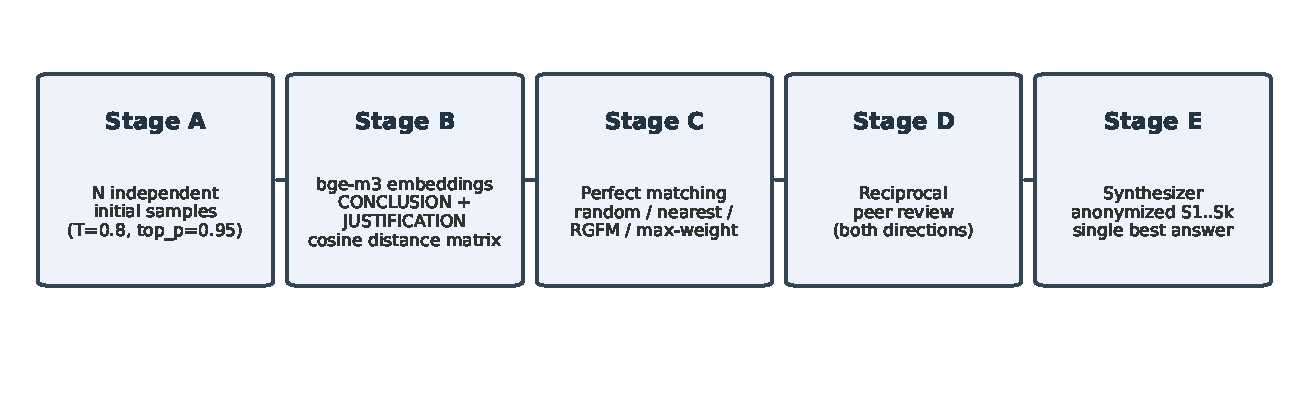
\includegraphics[width=0.9\textwidth]{../figures/F1_architecture.pdf}
\caption{流水线概览：$N$ 个缓存初始回答、bge-m3 距离矩阵、配对规则（随机 / 最近 / RGFM / 最大权重）、互惠配对限定互审，以及对全部回答与评审的最终合成。}
\label{fig:architecture}
\end{figure}

\subsection{总体准确率}

表~\ref{tab:mmlu-acc} 报告 MMLU-Pro 上的准确率（500 题 $\times$ 3 个实验种子，$n=1500$ 条合并观测）。所有 $N{=}4$ 聚合条件聚集在 0.8 个百分点的带内（0.837--0.845）；FPRR（C5，0.839）与算力匹配自审对照（C9，0.839）同处该带底部，比随机配对、最近配对、最大权重匹配与纯多数投票（均为 0.845）低 0.6 个百分点。图~\ref{fig:accuracy} 直观展示了这些几乎相同的准确率。

\begin{table}[t]
\centering
\small
\caption{MMLU-Pro 各条件准确率（500 题 $\times$ 3 种子；$n=1500$ 合并）。$95\%$ CI 为对题目的配对自助区间；各种子准确率各为 $n=500$。合并观测在种子间共享题目，因此 CI 轻度反保守；各种子数值呈现相同排序。}
\label{tab:mmlu-acc}
\begin{tabular}{llcccc}
\toprule
条件 & 名称 & 合并准确率 & 95\% CI & \multicolumn{2}{c}{各种子准确率} \\
\cmidrule(lr){5-6}
 & & & & s0 / s1 & s2 \\
\midrule
C0 & 单个回答            & 0.829 & [0.810, 0.848] & 0.824 / 0.834 & 0.830 \\
C1 & 多数投票            & 0.845 & [0.827, 0.863] & 0.844 / 0.844 & 0.848 \\
C2 & 集成 + 合成         & 0.837 & [0.818, 0.855] & 0.838 / 0.840 & 0.832 \\
C3 & 随机配对            & 0.845 & [0.827, 0.863] & 0.846 / 0.850 & 0.838 \\
C4 & 最近配对            & 0.845 & [0.827, 0.863] & 0.842 / 0.846 & 0.848 \\
C5 & FPRR (RGFM)         & 0.839 & [0.821, 0.857] & 0.844 / 0.836 & 0.838 \\
C6 & 最大权重匹配        & 0.845 & [0.826, 0.863] & 0.840 / 0.846 & 0.848 \\
C9 & 自审（算力匹配）    & 0.839 & [0.821, 0.857] & 0.838 / 0.838 & 0.842 \\
\bottomrule
\end{tabular}
\end{table}

\begin{table}[t]
\centering
\small
\caption{MMLU-Pro 上 C5（FPRR）与各对照的配对比较（$n=1500$）。diff = C5 减去对照，单位为百分点（pp）；CI = $95\%$ 配对自助区间；$p$ = 连续性校正 McNemar；$p_{\mathrm{Holm}}$ = 对主要族 \{C3, C4, C1, C9\} 的 Holm--Bonferroni 校正。中线以下为校正族之外的次要比较。}
\label{tab:mmlu-paired}
\begin{tabular}{lccccc}
\toprule
比较 & diff (pp) & 95\% CI (pp) & McNemar $b/c$ & $p$ & $p_{\mathrm{Holm}}$ \\
\midrule
C5 对 C3（随机）      & $-0.5$ & [$-1.3$, $0.2$] & 13/21 & 0.230 & 0.920 \\
C5 对 C4（最近）      & $-0.6$ & [$-1.5$, $0.3$] & 19/28 & 0.243 & 0.920 \\
C5 对 C1（投票）      & $-0.6$ & [$-1.5$, $0.3$] & 18/27 & 0.233 & 0.920 \\
C5 对 C9（自审）      & $0.0$  & [$-0.8$, $0.8$] & 19/19 & 0.871 & 0.920 \\
\midrule
C5 对 C0（单个）      & $+1.0$ & [$-0.1$, $2.1$] & 41/26 & 0.087 & --- \\
C5 对 C2（无互审）    & $+0.3$ & [$-0.7$, $1.2$] & 27/23 & 0.671 & --- \\
C5 对 C6（最大权重）  & $-0.5$ & [$-1.4$, $0.3$] & 16/24 & 0.268 & --- \\
\bottomrule
\end{tabular}
\end{table}

表~\ref{tab:mmlu-paired} 给出配对分析。每个主要比较的自助置信区间都跨零，四个 Holm 校正 $p$ 值全部为 $0.920$：FPRR 与随机配对（H1）、最近配对（H2）、多数投票（H3）或算力匹配自审对照之间均无可检测的差异。相对单回答基线，FPRR 提升 $+1.0$pp，但未达显著（$p=0.087$，未校正）。

SuperGPQA（500 题 $\times$ 4 种子，$n=2000$ 合并）在更低的准确率上讲述了同一个故事，且带有一处更尖锐的转折（表~\ref{tab:sg-acc}）。FPRR（0.599）与随机配对（0.606）、最近配对（0.605）、最大权重匹配（0.602）、多数投票（0.598）、自审（0.595）不可区分——甚至还略低；四个主要 Holm 校正 $p$ 值均 $\ge 0.987$（表~\ref{tab:sg-paired}）。在这个更难的基准上，每个 $N{=}4$ 条件都明显超过单回答基线（C0，0.561；C5 对 C0：$+3.8$pp，95\% CI [$+2.3$, $+5.2$]，$p<0.001$），因此集成机制本身确有收益。但无互审的合成器条件 C2（0.614）是最好的条件，且此处的损失不再是噪声：\textbf{C2 以 $1.5$pp 胜过 C5，自助置信区间不含零}（$[-2.6, -0.4]$，McNemar $p=0.010$；属 Holm 校正族之外的次要比较，且在跨种子相关性下是反保守的）。在更难的基准上，相对直接合成同一批缓存答案，互惠互审带来了虽小但统计上可检出的净损失——与 \S\ref{sec:btr} 的迁移分析一致（BTR $= 0.383$）。

\begin{table}[t]
\centering
\small
\caption{SuperGPQA 各条件准确率（500 题 $\times$ 4 种子；$n=2000$ 合并）。$95\%$ CI 为对题目的配对自助区间；各种子准确率各为 $n=500$。合并观测在种子间共享题目，因此 CI 轻度反保守；各种子数值呈现相同排序。}
\label{tab:sg-acc}
\begin{tabular}{llccc}
\toprule
条件 & 名称 & 合并准确率 & 95\% CI & 各种子准确率 (s0/s1/s2/s3) \\
\midrule
C0 & 单个回答            & 0.561 & [0.539, 0.583] & 0.546 / 0.572 / 0.568 / 0.558 \\
C1 & 多数投票            & 0.598 & [0.576, 0.619] & 0.594 / 0.604 / 0.588 / 0.604 \\
C2 & 集成 + 合成         & 0.614 & [0.593, 0.635] & 0.616 / 0.622 / 0.608 / 0.608 \\
C3 & 随机配对            & 0.606 & [0.584, 0.627] & 0.594 / 0.598 / 0.616 / 0.614 \\
C4 & 最近配对            & 0.605 & [0.583, 0.625] & 0.598 / 0.604 / 0.602 / 0.614 \\
C5 & FPRR (RGFM)         & 0.599 & [0.577, 0.620] & 0.598 / 0.602 / 0.596 / 0.598 \\
C6 & 最大权重匹配        & 0.602 & [0.580, 0.623] & 0.594 / 0.606 / 0.608 / 0.598 \\
C9 & 自审（算力匹配）    & 0.595 & [0.573, 0.616] & 0.602 / 0.586 / 0.588 / 0.604 \\
\bottomrule
\end{tabular}
\end{table}

\begin{table}[t]
\centering
\small
\caption{SuperGPQA 上 C5（FPRR）的配对比较（$n=2000$，4 个种子合并）。各列含义同表~\ref{tab:mmlu-paired}。注意次要比较 C5 对 C2：$-1.5$pp 且 CI 不含零（$p=0.010$，未校正）。}
\label{tab:sg-paired}
\begin{tabular}{lccccc}
\toprule
比较 & diff (pp) & 95\% CI (pp) & McNemar $b/c$ & $p$ & $p_{\mathrm{Holm}}$ \\
\midrule
C5 对 C3（随机）      & $-0.7$ & [$-1.8$, $+0.4$] & 56/70 & 0.247 & 0.987 \\
C5 对 C4（最近）      & $-0.6$ & [$-1.7$, $+0.5$] & 54/66 & 0.315 & 0.987 \\
C5 对 C1（投票）      & $+0.1$ & [$-1.1$, $+1.3$] & 72/70 & 0.933 & 1.000 \\
C5 对 C9（自审）      & $+0.4$ & [$-0.8$, $+1.5$] & 68/61 & 0.597 & 1.000 \\
\midrule
C5 对 C0（单个）      & $+3.8$ & [$+2.3$, $+5.2$] & 151/76 & $<$0.0001 & --- \\
C5 对 C2（无互审）    & $-1.5$ & [$-2.6$, $-0.4$] & 49/79 & 0.010 & --- \\
C5 对 C6（最大权重）  & $-0.3$ & [$-1.4$, $+0.8$] & 54/60 & 0.640 & --- \\
\bottomrule
\end{tabular}
\end{table}

\begin{figure}[t]
\centering
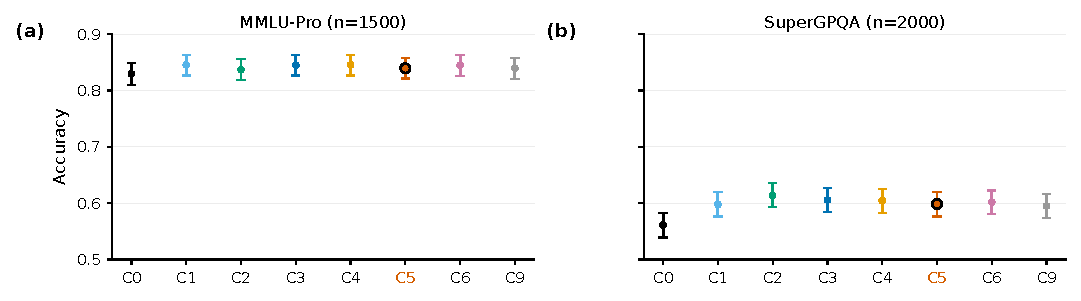
\includegraphics[width=0.85\textwidth]{../figures/F3_accuracy_by_condition.pdf}
\caption{两个基准上各条件的准确率（MMLU-Pro：$n=1500$，3 种子；SuperGPQA：$n=2000$，4 种子）。每个基准内所有 $N{=}4$ 条件在统计上不可区分，唯一例外是无互审合成（C2）在 SuperGPQA 上超过 FPRR。}
\label{fig:accuracy}
\end{figure}

\subsection{成本}

互审昂贵，且在此一无所获（表~\ref{tab:tokens}，图~\ref{fig:tokens}）。在 MMLU-Pro 上，C5 消耗 $11.89$M token——单回答基线的 $19.7\times$、多数投票的 $4.9\times$——准确率却比投票\emph{低} 0.6pp；每百万 token 的准确率从 1.37（C0）、0.35（C1）降至所有互审条件的 0.07。SuperGPQA 在每种子可比的 token 成本下呈现相同模式（C5 在 $4$ 个种子上共 $23.87$M），且互审还显著落后于无互审合成。

\begin{table}[t]
\centering
\small
\caption{总 token 用量与每百万 token 准确率（acc/Mtok；SuperGPQA 的 acc/Mtok 由合并总量计算）。SuperGPQA 列：$n=2000$，4 个种子合并。}
\label{tab:tokens}
\begin{tabular}{lcccc}
\toprule
 & \multicolumn{2}{c}{MMLU-Pro ($n=1500$)} & \multicolumn{2}{c}{SuperGPQA ($n=2000$)} \\
\cmidrule(lr){2-3}\cmidrule(lr){4-5}
条件 & tokens (M) & acc/Mtok & tokens (M) & acc/Mtok \\
\midrule
C0 & 0.60  & 1.37 & 1.20  & 0.47 \\
C1 & 2.41  & 0.35 & 4.76  & 0.13 \\
C2 & 3.82  & 0.22 & 8.14  & 0.08 \\
C3 & 11.80 & 0.07 & 23.77 & 0.03 \\
C4 & 11.78 & 0.07 & 23.74 & 0.03 \\
C5 & 11.89 & 0.07 & 23.87 & 0.03 \\
C6 & 11.95 & 0.07 & 23.92 & 0.03 \\
C9 & 11.26 & 0.07 & 22.71 & 0.03 \\
\bottomrule
\end{tabular}
\end{table}

\begin{figure}[t]
\centering
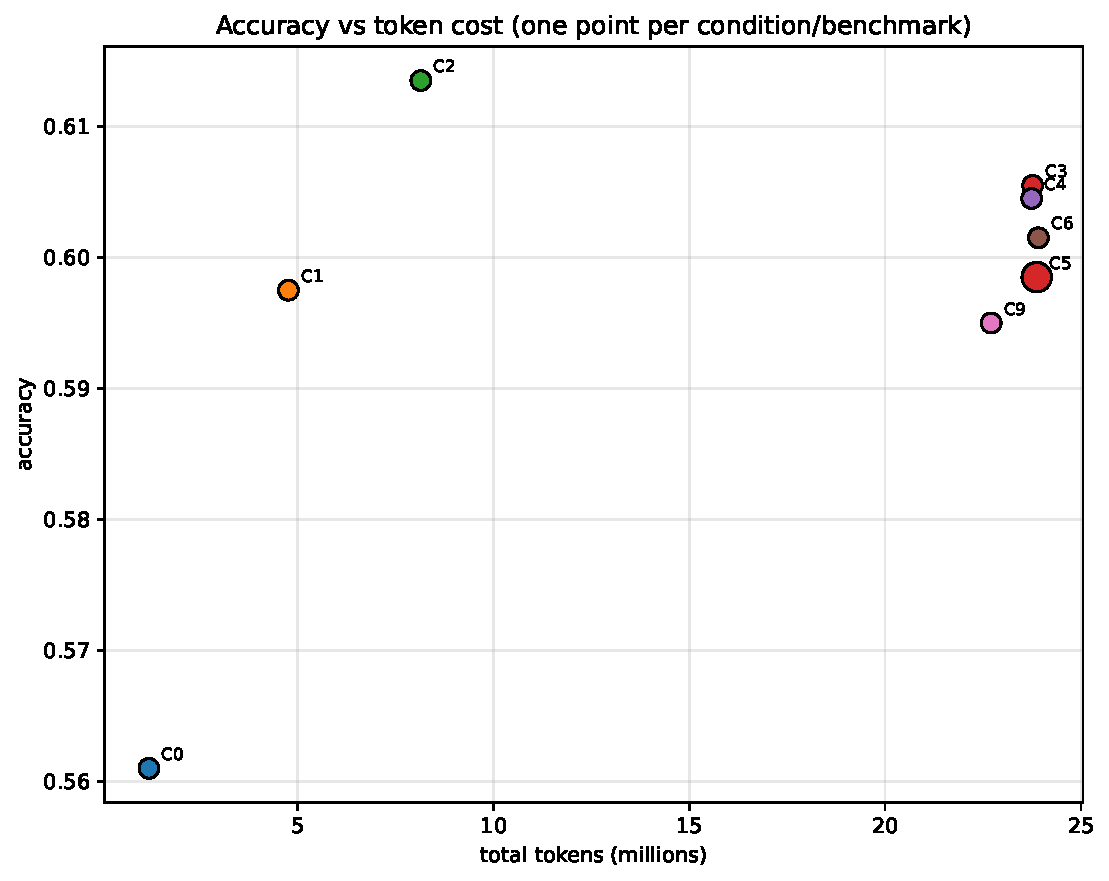
\includegraphics[width=0.85\textwidth]{../figures/F4_accuracy_vs_tokens.pdf}
\caption{准确率与总 token 消耗。互审条件（C3--C6, C9）占据一个昂贵的高原；投票（C1）在成本—准确率权衡上全面占优。}
\label{fig:tokens}
\end{figure}

\subsection{H1--H3 的裁定}

\textbf{H1（FPRR $>$ 随机配对）：不支持。} MMLU-Pro 上 $-0.5$pp，SuperGPQA 上 $-0.7$pp；两个 CI 均跨零（$p_{\mathrm{Holm}} = 0.920$ / $0.987$）。
\textbf{H2（FPRR $>$ 最近配对）：不支持。} $-0.6$pp / $-0.6$pp（$p_{\mathrm{Holm}} = 0.920$ / $0.987$）。
\textbf{H3（FPRR $>$ 多数投票）：不支持。} $-0.6$pp / $+0.1$pp（$p_{\mathrm{Holm}} = 0.920$ / $1.000$）。
精确最大权重匹配（C6）不优于贪心 RGFM；算力匹配自审对照（C9）在两个基准上几乎精确复现 FPRR 的准确率，因此该零结果不能归因于匹配次优或互审算力本身。

\section{消融实验}
\label{sec:ablations}

\paragraph{配对规则（C3--C6，相同初始回答）。}
由于四个配对条件互审的是\emph{同一}批缓存初始回答，它们之间的任何准确率差异都只能归因于匹配本身。而这样的差异基本不存在：MMLU-Pro 上 C3/C4/C5/C6 为 0.845 / 0.845 / 0.839 / 0.845（离散度 0.6pp）；SuperGPQA（$n=2000$，4 种子）上为 0.606 / 0.605 / 0.599 / 0.602（离散度 0.7pp）。精确最大权重匹配（C6）与贪心 RGFM（C5）不可区分；极性相反的最近配对（C4）与随机配对持平。图~\ref{fig:matchings} 直观展示四种规则如何以截然不同的方式连接同一批回答；连线方式对准确率没有影响。

\begin{figure}[t]
\centering
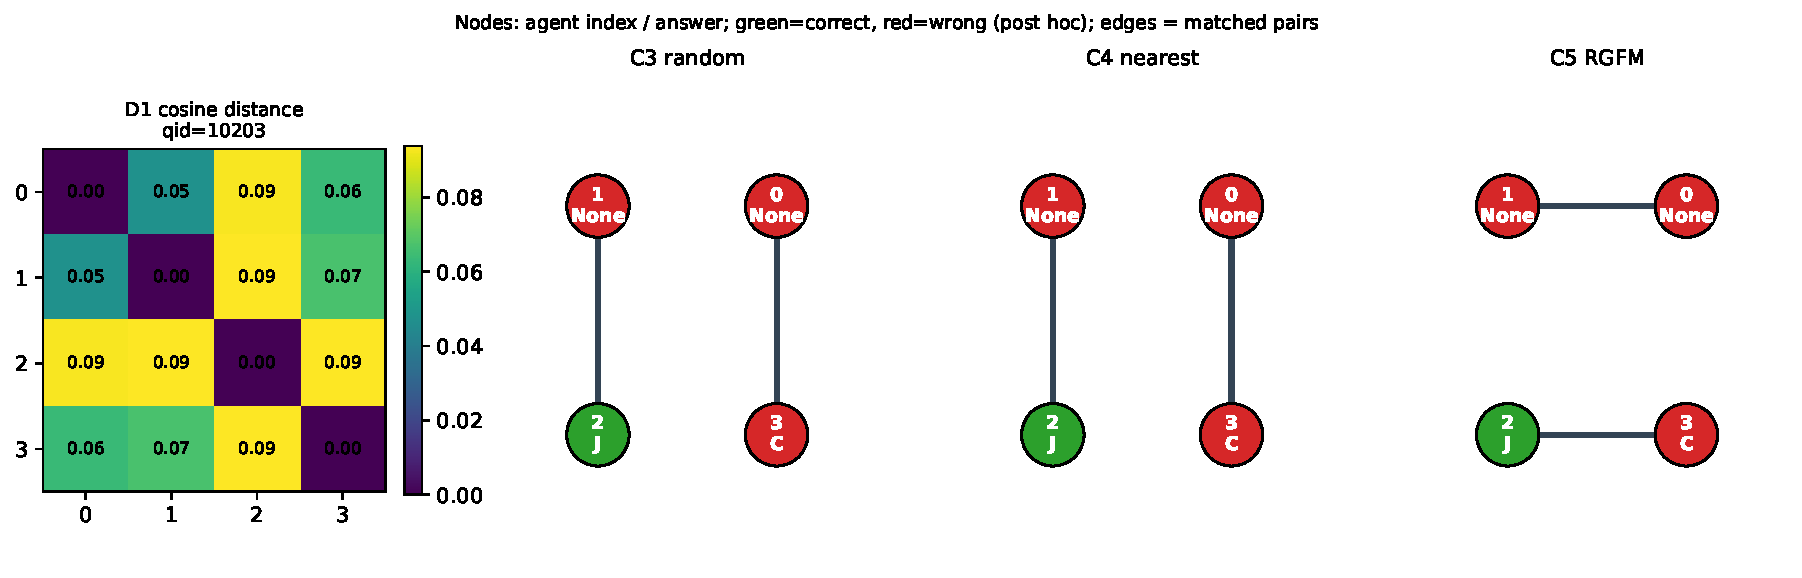
\includegraphics[width=0.48\textwidth]{../figures/F2_distance_matchings_mmlu_pro.pdf}\hfill
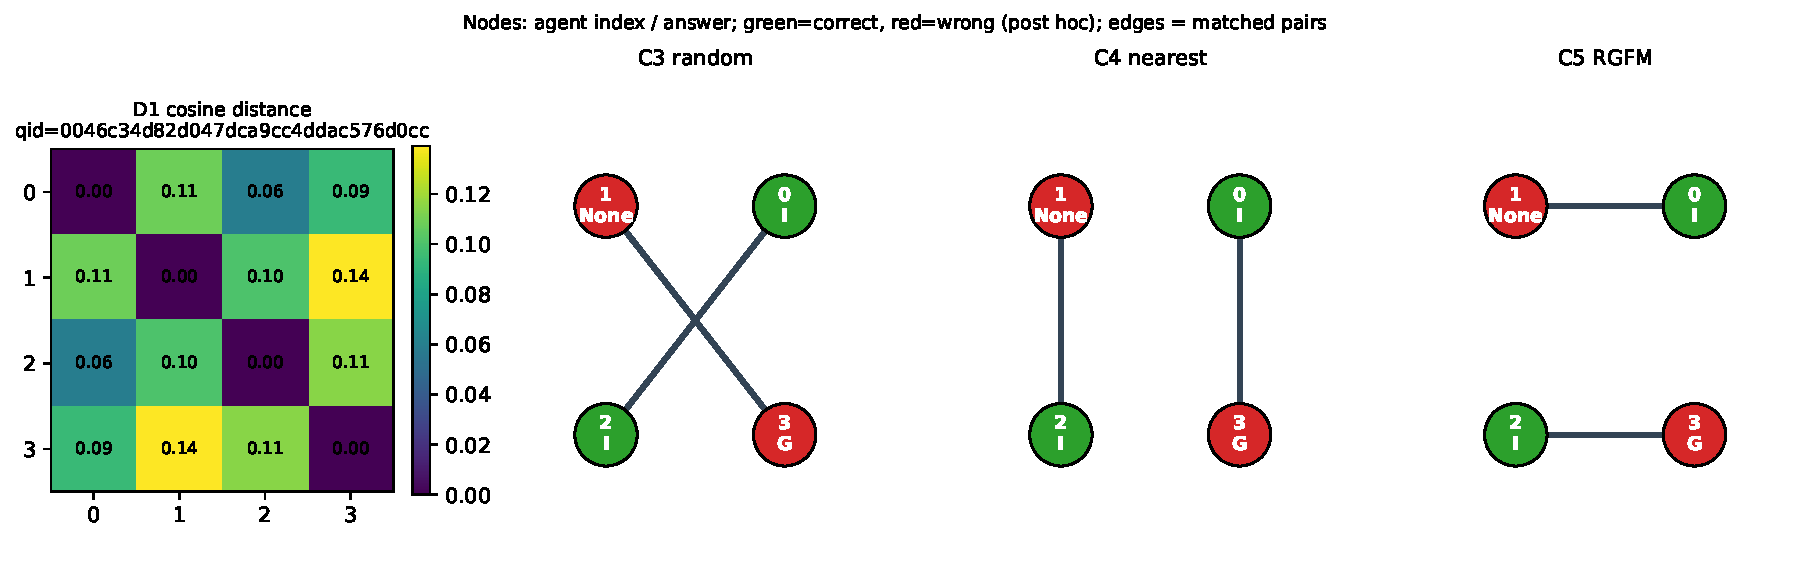
\includegraphics[width=0.48\textwidth]{../figures/F2_distance_matchings_supergpqa.pdf}
\caption{距离矩阵，以及随机 / 最近 / RGFM / 最大权重在相同回答集上诱导的匹配（左：MMLU-Pro；右：SuperGPQA，图中展示种子 0 作为示例；合并结果见表~\ref{tab:mmlu-acc} 与 \ref{tab:sg-acc}）。}
\label{fig:matchings}
\end{figure}

\paragraph{互审与不互审（C2）、合成器与投票（C1）。}
在 MMLU-Pro 上，互审条件（0.839--0.845）与无互审合成器条件 C2（0.837）相差在 0.8pp 以内，C1 投票（0.845）以极低得多的成本追平最好的互审条件。在 SuperGPQA 上排序反转：C2（0.614）是最好的条件，\emph{高于}所有互审条件（0.599--0.606），C1 为 0.598——且四个种子下差距在统计上可检出（C5 对 C2：$-1.5$pp，95\% CI [$-2.6$, $-0.4$]，$p=0.010$ 未校正；表~\ref{tab:sg-paired}）。因此，互惠互审相对任何一个聚合基线都不增值——在更难的基准上反而略有减值。

\paragraph{算力匹配（C9）。}
相同调用预算下的自审几乎精确复现 FPRR（MMLU-Pro 0.839 对 0.839；SuperGPQA 0.595 对 0.599；C5 对 C9 差值 $0.0$pp / $+0.4$pp，$p_{\mathrm{Holm}} = 0.920$ / $1.000$）。把互审预算花在自我批评上与花在同伴互审上恰好一样好——也一样有限，因此该零结果是\emph{路由}的零结果，而非预算的零结果。

\paragraph{距离度量（D1--D4）与预实验 $\lambda$。}
按预注册，混合距离 D3 的 $\lambda$ 在完整运行之前固定为 $0.5$（它是余量更高基准上的预实验最优值，其余情形下取中点；C5 下的预实验距离消融，每基准 100 题，种子 0；预实验数据仅用于调参，不作为证据报告）。表~\ref{tab:dist-ablation} 报告完整的 200 题距离消融（D2/D3/D4 下的 C5，种子 0；每个基准内 D3/D4 复用 D2 的缓存初始回答，因此跨度量的配对比较分离了各度量所诱导的拓扑）。该分析是\emph{探索性}的（预注册修订案 8：机制性分析，位于 Holm 校正主要族之外）。

在 SuperGPQA 上，感知分歧的度量优于纯语义距离：D4（NLI 矛盾）达 $0.680$，D2（结论+理由余弦）为 $0.650$，配对差值 D4 $-$ D2 为 $+3.0$pp，自助 CI 不含零（$[+0.5, +6.0]$）——但仅有 $7$ 对 $1$ 道不一致题目（McNemar $p=0.077$）、单种子、200 题：信号真实但脆弱，需要复现。机制与 \S\ref{sec:mechanism} 一致：D4 下多数腐化率较 D2 下降六倍（$0.008$ 对 $0.048$；D3：$0.024$），而纠正率是三种度量中最高的（$0.289$ 对 D2 的 $0.268$；互审级错误反对裁定率持平，$0.047$--$0.052$）——NLI 矛盾比嵌入余弦更接近\emph{认识上的}对立，因此 D4 下的最远配对挑起的争执更经常值得一吵。在 MMLU-Pro 上所有度量差异均为零（D2/D3 彼此之间以及与投票的差距均在 $0.5$pp 以内）：饱和的基准没有为任何路由信号留下余量。MMLU-Pro D4 未运行（预算）。

\begin{table}[t]
\centering
\small
\begin{tabular}{llcccc}
\hline
基准 & 度量 & C5 准确率 & C1 准确率 & C5 $-$ C1 [95\% CI], $p$ & 与 D2 配对 [95\% CI], $p$ \\
\hline
SuperGPQA & D2（余弦）        & 0.650 [0.585, 0.715] & 0.630 & $+2.0$ [$-2.0$, $+6.0$], $0.45$  & --- \\
SuperGPQA & D3 $\lambda{=}0.5$ & 0.670 [0.605, 0.735] & 0.630 & $+4.0$ [$+0.5$, $+7.5$], $0.061$ & $+2.0$ [$-0.5$, $+5.0$], $0.29$ \\
SuperGPQA & D4（NLI 矛盾）    & 0.680 [0.615, 0.745] & 0.630 & $+5.0$ [$+2.0$, $+8.5$], $0.009$ & $+3.0$ [$+0.5$, $+6.0$], $0.077$ (7:1) \\
MMLU-Pro  & D2（余弦）        & 0.860 [0.810, 0.905] & 0.865 & $-0.5$ [$-2.5$, $+1.5$], NS      & --- \\
MMLU-Pro  & D3 $\lambda{=}0.5$ & 0.865 [0.815, 0.910] & 0.865 & $0.0$ [$-2.5$, $+3.0$], NS       & $+0.5$ [$-1.5$, $+2.5$], $1.0$ \\
MMLU-Pro  & D4（NLI 矛盾）    & \multicolumn{4}{c}{\emph{未运行（预算）}} \\
\hline
\end{tabular}
\caption{C5 下的距离度量消融（每基准 200 题，种子 0；探索性，修订案 8）。每个基准内所有度量互审完全相同的缓存初始回答，因此配对差值分离了度量诱导的拓扑。C1（多数投票）在相同回答集上计算。差值单位为百分点；$p$ 值为连续性校正 McNemar，未校正。}
\label{tab:dist-ablation}
\end{table}

\paragraph{智能体数量 $N$ 与配对种子方差。}
未运行（预算）。$N \in \{2,6,8\}$ 消融与配对种子方差研究（C3/C5 的配对种子 1、2，MMLU-Pro 200 题子集）已在预注册中设计并冻结（修订案 8），但未能在剩余 API 预算内执行；我们将其如实报告为缺失而非默默丢弃，并将其缺失计为一项局限（\S\ref{sec:limitations}）。

\section{机制分析}
\label{sec:mechanism}

总体零结果引出一个更尖锐的问题：异配边是否携带\emph{任何}额外信号？若有，它死在哪里？我们将互审阶段分解为两条方向相反的链（图~\ref{fig:funnels}）：\emph{正向链}——题目至少有一个错误初始答案（E0），互审者检出该错误（E1），提出正确修复（E2），最终答案正确（E3）；\emph{反向链}——题目至少有一个正确初始答案（C0），互审者错误反对正确的同伴（C1），正确的互审者失稳而更改或怀疑有效答案（C2），最终答案错误（C3）。

\begin{figure}[t]
\centering
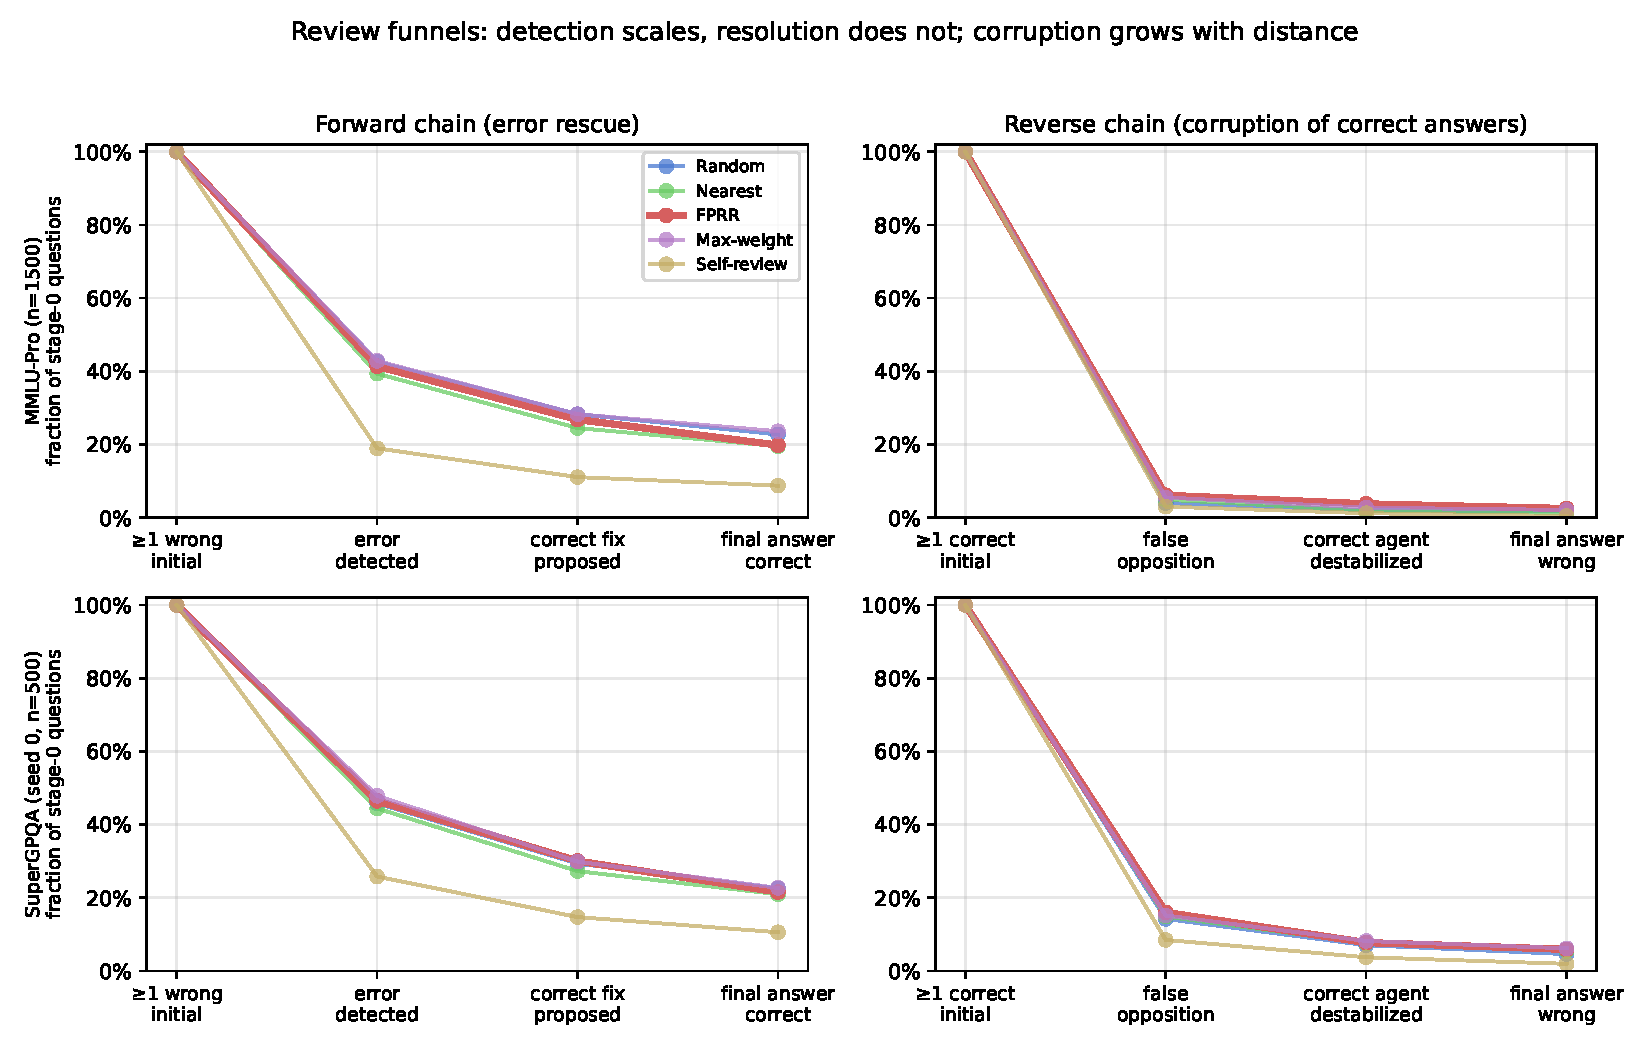
\includegraphics[width=0.95\textwidth]{../figures/F8_repair_funnels.pdf}
\caption{两个基准上的双层题目级漏斗（MMLU-Pro：$n=1500$，3 种子；SuperGPQA：$n=2000$，4 种子）。正向链 E0$\to$E3（错误暴露 $\to$ 检出 $\to$ 提出修复 $\to$ 最终正确）与反向链 C0$\to$C3（存在正确答案 $\to$ 错误反对 $\to$ 失稳 $\to$ 最终错误）。检出随配对距离上升；解决不随距离上升；反向链在异配配对下变得更重。}
\label{fig:funnels}
\end{figure}

\subsection{正向链：距离买来错误暴露}
\label{sec:fwd}

FPRR 确实把互审流量转移到可能发生分歧的配对上。按互审者—被审者正误统计有向互审，C5 将 $412/6000$（$6.9\%$）的 MMLU-Pro 互审置于正误混合的配对上，随机配对为 $328$（$5.5\%$），最近配对为 $320$（$5.3\%$）——跨错误边相对增加 $25$--$30\%$，与精确最大权重匹配持平（C6：$416$，$6.9\%$）。SuperGPQA 上转移更小：C5 将 $1270/8000$（$15.9\%$）的互审置于混合配对，随机配对为 $1194$（$14.9\%$），最近配对为 $1098$（$13.7\%$）（C6：$1330$，$16.6\%$）。

表~\ref{tab:deciles} 将 C5 全部互审按配对距离十分位分层，表~\ref{tab:review-outcomes} 给出总体互审级结果。在两个基准、全部四种配对规则下，检出率随距离陡峭上升，仅有小幅局部非单调（图~\ref{fig:deciles}）：C5 下，P（裁定 \texttt{INCORRECT} $\mid$ 被审者错误）在 MMLU-Pro 上从最低十分位的 $0.000$ 升至最高十分位的 $0.379$，在 SuperGPQA 上从 $0.050$ 升至 $0.361$；C3--C6 最高十分位检出率横跨 $0.368$--$0.436$（MMLU-Pro）与 $0.301$--$0.361$（SuperGPQA）。互审对错误答案的检出也远高于自审（C9：$0.091$ / $0.135$，C3--C6 为 $0.19$--$0.26$）。注意在 MMLU-Pro 上取得最高检出率的是 C6 而非 C5（$0.227$），但它与 C3/C4 的准确率持平：超出随机基线的额外检出在任何路由规则下都没有总体回报。

\begin{table}[t]
\centering
\small
\caption{两个基准上 C5（FPRR）按配对距离十分位分层的互审行为（MMLU-Pro：6000 条互审；SuperGPQA：8000 条互审，4 种子）。det = P（裁定 \texttt{INCORRECT} $\mid$ 被审者错误）；cor = P（错误被纠正 $\mid$ 被审者错误）；f.o. = P（错误反对 $\mid$ 被审者正确）。十分位区间为余弦距离；边在 C3--C6 上合并。}
\label{tab:deciles}
\begin{tabular}{ccccccccc}
\toprule
 & \multicolumn{4}{c}{MMLU-Pro (6000 条互审)} & \multicolumn{4}{c}{SuperGPQA (8000 条互审)} \\
\cmidrule(lr){2-5}\cmidrule(lr){6-9}
十分位 & 距离区间 & det & cor & f.o. & 距离区间 & det & cor & f.o. \\
\midrule
1  & [0.000, 0.028] & 0.000 & 0.000 & 0.002 & [0.000, 0.034] & 0.050 & 0.021 & 0.027 \\
2  & [0.028, 0.043] & 0.073 & 0.018 & 0.002 & [0.034, 0.051] & 0.083 & 0.026 & 0.018 \\
3  & [0.043, 0.056] & 0.089 & 0.051 & 0.006 & [0.051, 0.066] & 0.178 & 0.079 & 0.030 \\
4  & [0.056, 0.069] & 0.089 & 0.013 & 0.009 & [0.066, 0.078] & 0.233 & 0.123 & 0.039 \\
5  & [0.069, 0.081] & 0.105 & 0.058 & 0.016 & [0.078, 0.090] & 0.229 & 0.139 & 0.079 \\
6  & [0.081, 0.094] & 0.200 & 0.130 & 0.023 & [0.090, 0.104] & 0.258 & 0.129 & 0.065 \\
7  & [0.094, 0.111] & 0.156 & 0.094 & 0.013 & [0.104, 0.119] & 0.279 & 0.155 & 0.072 \\
8  & [0.111, 0.130] & 0.236 & 0.127 & 0.030 & [0.119, 0.138] & 0.262 & 0.139 & 0.100 \\
9  & [0.130, 0.161] & 0.256 & 0.103 & 0.043 & [0.138, 0.168] & 0.268 & 0.151 & 0.090 \\
10 & [0.161, 1.000] & 0.379 & 0.209 & 0.051 & [0.168, 1.000] & 0.361 & 0.171 & 0.097 \\
\bottomrule
\end{tabular}
\end{table}

\begin{table}[t]
\centering
\small
\caption{互审级结果。det = P（裁定 \texttt{INCORRECT} $\mid$ 被审者错误）；f.o. = P（错误反对 $\mid$ 被审者正确）。SuperGPQA：$n=2000$，4 种子。}
\label{tab:review-outcomes}
\begin{tabular}{lcccccc}
\toprule
 & \multicolumn{3}{c}{MMLU-Pro} & \multicolumn{3}{c}{SuperGPQA (4 种子)} \\
\cmidrule(lr){2-4}\cmidrule(lr){5-7}
条件 & $n$ 条互审 & det & f.o. & $n$ 条互审 & det & f.o. \\
\midrule
C3 随机      & 5928 & 0.202 & 0.012 & 7561 & 0.241 & 0.054 \\
C4 最近      & 5918 & 0.192 & 0.016 & 7568 & 0.231 & 0.057 \\
C5 FPRR      & 5912 & 0.212 & 0.020 & 7570 & 0.256 & 0.063 \\
C6 最大权重  & 5902 & 0.227 & 0.018 & 7561 & 0.254 & 0.062 \\
C9 自审      & 5943 & 0.091 & 0.009 & 7668 & 0.135 & 0.037 \\
\bottomrule
\end{tabular}
\end{table}

\begin{figure}[t]
\centering
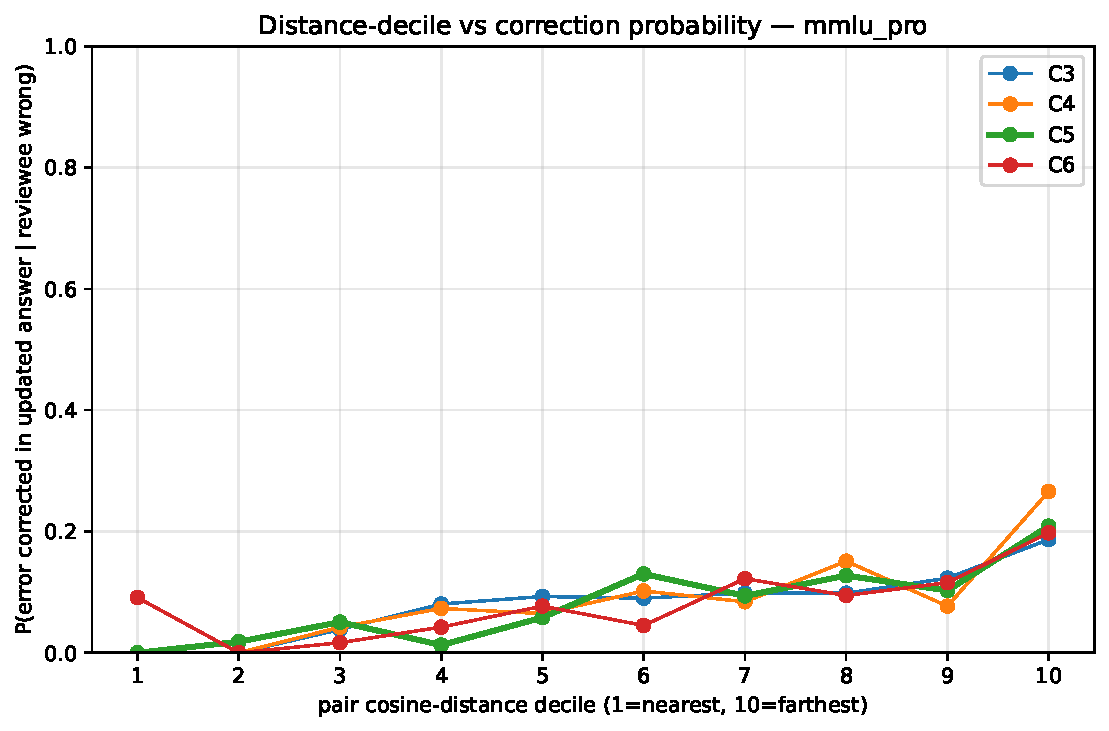
\includegraphics[width=0.48\textwidth]{../figures/F5_decile_correction_mmlu_pro.pdf}\hfill
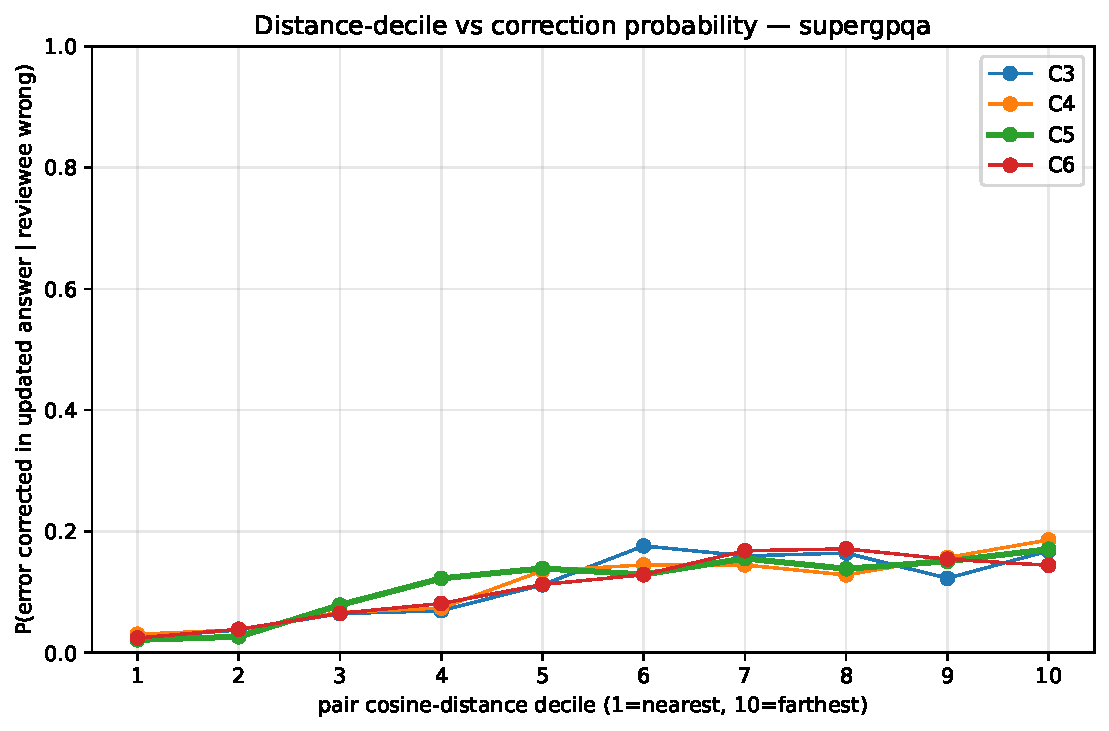
\includegraphics[width=0.48\textwidth]{../figures/F5_decile_correction_supergpqa.pdf}
\caption{C3--C6 按配对距离十分位的检出率、纠正率与错误反对率（左：MMLU-Pro；右：SuperGPQA，$n=2000$，4 种子）。每种配对规则下检出率随距离上升；纠正率饱和；错误反对率攀升。}
\label{fig:deciles}
\end{figure}

\paragraph{分阶段回归：错误暴露与解决。}
为定位距离\emph{究竟}作用于何处，我们在配对距离上拟合三个 logistic 回归（C3--C6 合并互审）：检出错误的被审者、在检出条件下提出正确修复、在存在修复条件下最终答案正确（表~\ref{tab:stage-reg}）。MMLU-Pro 上只有检出阶段对距离敏感（$\beta = +12.2$，$p<0.0001$）；向修复（$p=0.20$）与采纳（$p=0.84$）的传播是平的。SuperGPQA 上三个阶段全部显著（$\beta = +7.5$、$+1.7$、$+7.3$；$p$ 分别为 $<0.0001$、$0.016$、$<0.0001$）——距离在那里确实传播到了解决——但总体准确率仍不动，因为反向链（\S\ref{sec:rev}）随同一距离放大。因此精确的陈述是：\emph{距离改善错误暴露；错误暴露是否传播为解决，取决于具体情形。}

\begin{table}[t]
\centering
\small
\caption{正向链事件对配对余弦距离的分阶段 logistic 回归（C3--C6 合并互审；SuperGPQA：4 种子）。}
\label{tab:stage-reg}
\begin{tabular}{llccc}
\toprule
基准 & 阶段（结果） & $n$ & $\beta_{\mathrm{dist}}$ (SE) & $p$ \\
\midrule
MMLU-Pro & P（检出 $\mid$ 被审者错误）        & 4040 & $+12.20$ (0.75) & $<0.0001$ \\
MMLU-Pro & P（正确修复 $\mid$ 已检出）       & 796  & $+1.64$ (1.29)  & $0.203$ \\
MMLU-Pro & P（最终正确 $\mid$ 存在修复）     & 321  & $-0.52$ (2.66)  & $0.844$ \\
\midrule
SuperGPQA & P（检出 $\mid$ 被审者错误）      & 14124 & $+7.54$ (0.37) & $<0.0001$ \\
SuperGPQA & P（正确修复 $\mid$ 已检出）      & 3161  & $+1.68$ (0.70) & $0.016$ \\
SuperGPQA & P（最终正确 $\mid$ 存在修复）    & 1224  & $+7.30$ (1.52) & $<0.0001$ \\
\bottomrule
\end{tabular}
\end{table}

\subsection{互审超过初始回答候选选择神谕——但几乎无法交付}
\label{sec:oracle}

\emph{初始回答候选选择神谕}——总是从四个缓存初始答案中选出最佳者——在 MMLU-Pro 上可得 $0.883$、在 SuperGPQA 上可得 $0.697$，而最佳实际条件为 $0.845$ 与 $0.614$（差距约 $3.7$pp 与 $8.3$pp，按未舍入值 $0.8827$ 对 $0.8453$、$0.6965$ 对 $0.614$ 计算；表中的舍入值显示 $3.8$pp）。同期工作在更大规模上得到相同诊断：跨 15{,}336 道题、81{,}390 个固定候选池，Ji 等~\cite{ji2026candidate} 表明正确答案经常存在于候选集中却未被选中，且裁判可靠性随任务、生成者与正确答案的稀有度而变化。我们的候选选择神谕差距在完全受控的相同回答集下证实了这一候选供给瓶颈，并通过度量互审在候选池\emph{之外}新增了什么而将其进一步推进。然而，该神谕\emph{不是}审议系统的上限，因为互审者可以产生初始集 $R_x$ 之外的答案。他们确实做到了：在四个初始答案全错的题目上（MMLU-Pro 176/1500，$11.7\%$；SuperGPQA 607/2000，$30.4\%$），互审在 $0$--$2.3\%$（MMLU-Pro）与 $3.1$--$4.1\%$（SuperGPQA）的情形下（跨条件）产生了 $R_x$ 之外的正确答案——互审阶段的输出在经验上不只是初始答案的函数。

但交付正是这些新信息死亡之处（表~\ref{tab:delivery}）。端到端看，新颖正确提议进入最终答案的比例为：MMLU-Pro 上 C5 为 $1/176$ 题（$0.6\%$），SuperGPQA 上至多 $9/607$（$1.5\%$）（C9；C5：$8/607 = 1.3\%$）；「提出未交付」列量化了这一损失——例如 C3 在 MMLU-Pro 上提出 $4$ 个新颖正确答案但交付为零，C5 在 SuperGPQA 上提出 $25$ 个但仅采纳 $6$ 个（损失 $19$ 个）。在一致全错子集（120 与 401 题）内，每个条件的最终答案在至少 $99.2\%$（MMLU-Pro）与 $98.0\%$（SuperGPQA）的情形下仍然错误：互审能\emph{创造}缺失的答案，但流水线无法\emph{识别}它。

\begin{table}[t]
\centering
\small
\caption{全错题上的新颖正确交付审计（四个初始答案全错；MMLU-Pro：176 题，3 种子；SuperGPQA：607 题，4 种子）。新颖提出 = 互审提出了初始集中没有的正确答案；最终正确 = 题目最终答对；提出未交付 = 已提出但未被采纳进入最终答案。}
\label{tab:delivery}
\begin{tabular}{lcccccccc}
\toprule
 & \multicolumn{4}{c}{MMLU-Pro} & \multicolumn{4}{c}{SuperGPQA (4 种子)} \\
\cmidrule(lr){2-5}\cmidrule(lr){6-9}
条件 & 新颖提出 & 最终正确 & 被采纳 & 提出未交付 & 新颖提出 & 最终正确 & 被采纳 & 提出未交付 \\
\midrule
C3 & 4 & 0 & 0 & 4 & 21 & 8 & 7 & 14 \\
C4 & 3 & 0 & 0 & 3 & 20 & 8 & 6 & 14 \\
C5 & 2 & 1 & 1 & 1 & 25 & 8 & 6 & 19 \\
C6 & 0 & 0 & 0 & 0 & 19 & 7 & 6 & 13 \\
C9 & 1 & 0 & 0 & 1 & 21 & 9 & 8 & 13 \\
\bottomrule
\end{tabular}
\end{table}

\subsection{反向链：失稳，而非离群放大}
\label{sec:rev}

我们在预实验时期对正确多数腐化的工作解释是\emph{离群放大}：最远配对优先把唯一的错误离群答案接到某个正确智能体上。完整数据否定了它作为总体机制的地位。在 3:1 的答案分裂中——通过只比较具有相同分裂结构的题目来控制题目难度——单例答案正确的概率确实远低于多数（MMLU-Pro 上 $20.8\%$ 对 $57.6\%$；SuperGPQA 上 $28.4\%$ 对 $44.7\%$）：遥远、反常的答案不成比例地错误。但每题\emph{最大距离}边的两个端点出错的概率基本等于基准率（MMLU-Pro：$17.1\%$ 对最小距离边的 $16.3\%$，基准率 $16.8\%$；SuperGPQA：$44.7\%$ 对 $43.6\%$，基准率 $44.1\%$）：最远配对\emph{并不}系统性地选择错误伙伴。因此我们不再把离群放大当作总体解释；3:1 结果仅保留为「离群答案准确率低」，而非「FPRR 选了坏伙伴」。

反向链实际展示的是\emph{错误反对与有效答案失稳}。错误反对随配对距离上升（表~\ref{tab:deciles}：MMLU-Pro C5 下从 $0.002$ 升至 $0.051$；SuperGPQA 最大权重配对下最高 $0.104$）。在题目层面（图~\ref{fig:funnels}，C 侧），MMLU-Pro 上 C5 下正确互审者的失稳比 C3 更重（$50/1324 = 4\%$ 对 $27/1324 = 2\%$；最终转错 $33$ 对 $23$）——C5 位于 MMLU-Pro 反向漏斗的顶端——而 SuperGPQA 上所有互审条件的反向链都很重（失稳 $0.07$--$0.08$）。语义不相似并没有把互审路由到错误伙伴；它制造的是对正确答案的反对。

预注册的次要指标（表~\ref{tab:secondary}）与共识迁移（图~\ref{fig:transitions}）量化了由此产生的平衡。互审条件比投票更经常地挽回多数错误——但在 MMLU-Pro 上名义最好的是\emph{随机}配对而非 FPRR（挽回率 $0.099$；营救率 $0.082$）；在 SuperGPQA 上无互审合成器 C2（$0.099$ / $0.100$）在没有任何互审的情况下追平最好的互审条件（C4：$0.098$ / $0.106$），而 C5 是除 C9 外最弱的互审条件（$0.089$ / $0.096$）。相对 0 号智能体的初始答案，MMLU-Pro 互审条件把 $15.2$--$18.0\%$ 的初始错误情形翻正，同时腐化 $1.5$--$2.1\%$ 的初始正确情形（C5：$16.0\%$ / $2.1\%$；C1 投票：$11.7\%$ / $0.5\%$）；SuperGPQA 上这一权衡几乎对称（C5：$17.2\%$ 对 $6.8\%$）——这正是更难的基准上没有任何净收益得以实现的原因。

\begin{table}[t]
\centering
\small
\caption{次要指标（各条件比率）。rec = 多数错误挽回率；cor = 正确多数腐化率；res = 少数派营救率。SuperGPQA：$n=2000$，4 种子。}
\label{tab:secondary}
\begin{tabular}{lcccccc}
\toprule
 & \multicolumn{3}{c}{MMLU-Pro} & \multicolumn{3}{c}{SuperGPQA (4 种子)} \\
\cmidrule(lr){2-4}\cmidrule(lr){5-7}
条件 & rec & cor & res & rec & cor & res \\
\midrule
C0 & 0.026 & 0.024 & 0.032 & 0.048 & 0.094 & 0.064 \\
C2 & 0.065 & 0.022 & 0.050 & 0.099 & 0.040 & 0.100 \\
C3 & 0.099 & 0.019 & 0.082 & 0.096 & 0.051 & 0.100 \\
C4 & 0.086 & 0.016 & 0.059 & 0.098 & 0.054 & 0.106 \\
C5 & 0.078 & 0.021 & 0.059 & 0.089 & 0.059 & 0.096 \\
C6 & 0.086 & 0.017 & 0.064 & 0.096 & 0.058 & 0.099 \\
C9 & 0.065 & 0.019 & 0.036 & 0.070 & 0.051 & 0.075 \\
\bottomrule
\end{tabular}
\end{table}

\begin{figure}[t]
\centering
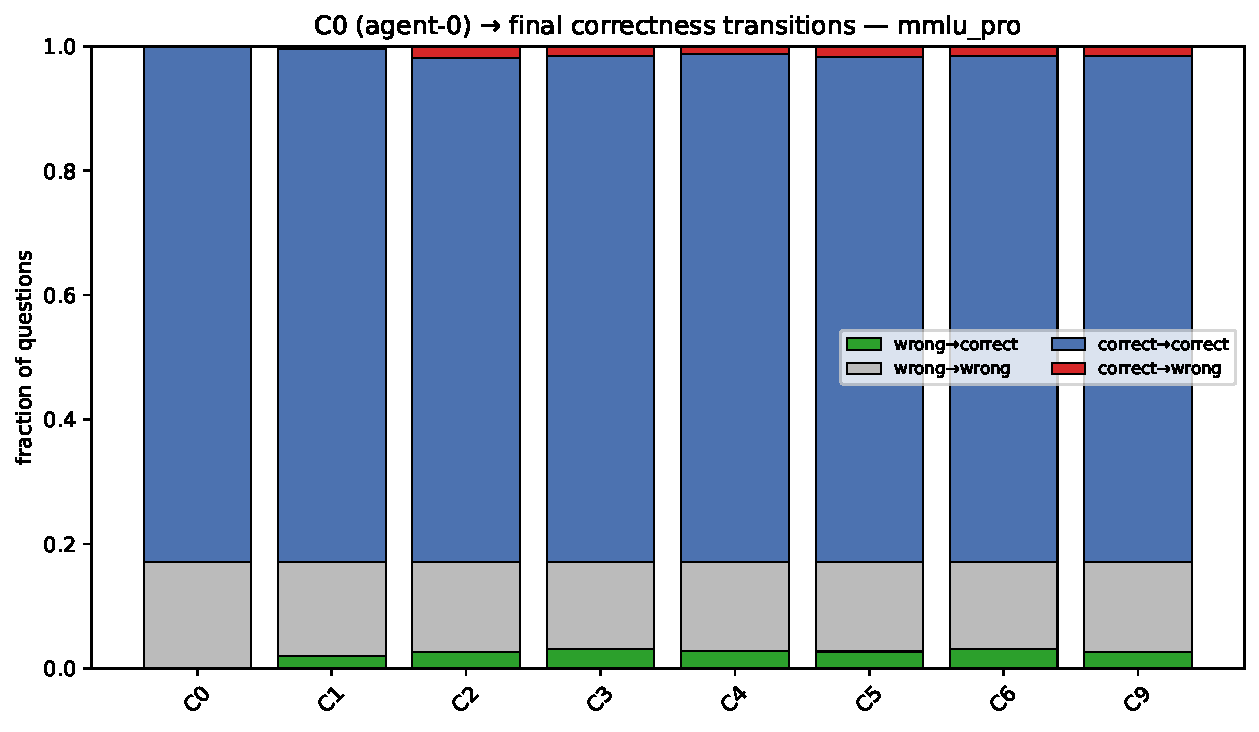
\includegraphics[width=0.48\textwidth]{../figures/F6_error_transitions_mmlu_pro.pdf}\hfill
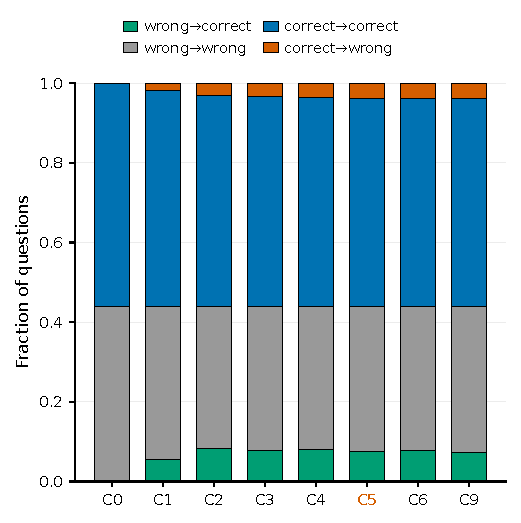
\includegraphics[width=0.48\textwidth]{../figures/F6_error_transitions_supergpqa.pdf}
\caption{相对 0 号智能体初始答案的错误迁移（左：MMLU-Pro；右：SuperGPQA，$n=2000$，4 种子）。在每种互审拓扑下，挽回与腐化几乎相互抵消。}
\label{fig:transitions}
\end{figure}

\subsection{互审活跃但净零：有益迁移率}
\label{sec:btr}

C5 与自审对照 C9 准确率持平，可能意味着互审是冗余的——也可能意味着它在两个方向上都活跃并相互抵消。C2$\leftrightarrow$C5 的题目级迁移给出了裁决：在同一合成流水线上加入互审，把 $27$ 道 MMLU-Pro 题目从错翻正、$23$ 道从正翻错（净 $+4$；$1450$ 道不变），SuperGPQA 上为 $49$ 对 $79$（净 $-30$；$1872$ 道不变）。互审是\emph{活跃}的，且在 SuperGPQA 上活跃地为净负——与表~\ref{tab:sg-paired} 中显著的 C2 $>$ C5 差距互为镜像。我们将其概括为\textbf{有益迁移率}，$\mathrm{BTR} = \#\text{获救} / (\#\text{获救} + \#\text{受害})$：MMLU-Pro 上 $0.54$，SuperGPQA 上 $0.383$。（BTR 由 C2 与 C5 的逐题迁移计数计算；它不是对所有答案修改事件的精度，后者需要对每一次互审引起的编辑做单独审计。）

\subsection{拓扑有处理作用的子集}
\label{sec:subsets}

有一种稀释批评认为，总体零结果不提供信息，因为大多数题目的答案一致，任何拓扑都无从作用。因此我们限制到\emph{分歧子集}（初始答案不一致；MMLU-Pro 上 $223$ 题，$14.9\%$；SuperGPQA 上 $754$ 题，$37.7\%$）与\emph{可挽回子集}（正确答案出现在初始回答中的分歧题；$59$ 题，$3.9\%$；与 $234$ 题，$11.7\%$）。表~\ref{tab:subsets} 驳回了稀释反驳，但也不支持任何条件性论断：C5 在两个基准上都\emph{落后}于 C3——在 MMLU-Pro 分歧子集与可挽回子集上分别落后 $3.1$pp 与 $13.6$pp，在对应的 SuperGPQA 子集上落后 $2.0$pp 与 $1.7$pp（SuperGPQA 可挽回子集上 C5 对 C4：$-3.4$pp）。方向在两个基准上一致为负，但每个置信区间都跨零——在拓扑有空间发挥作用之处，FPRR 没有表现出收益，只有一致的、不显著的惩罚。

\begin{table}[t]
\centering
\small
\caption{在配对拓扑能够发挥作用的子集上 C5 与 C3 的比较（配对自助 CI；SuperGPQA：$n=2000$，4 种子）。}
\label{tab:subsets}
\begin{tabular}{llccccc}
\toprule
基准 & 子集 & $n$ & C3 准确率 & C5 准确率 & C5$-$C3 (pp) & 95\% CI (pp) \\
\midrule
MMLU-Pro & 分歧    & 223 & 0.498 & 0.466 & $-3.1$ & [$-8.1$, $+1.8$] \\
MMLU-Pro & 可挽回  & 59  & 0.475 & 0.339 & $-13.6$ & [$-25.4$, $+0.0$] \\
SuperGPQA & 分歧   & 754 & 0.488 & 0.468 & $-2.0$ & [$-4.8$, $+0.8$] \\
SuperGPQA & 可挽回 & 234 & 0.402 & 0.385 & $-1.7$ & [$-8.6$, $+5.1$] \\
\bottomrule
\end{tabular}
\end{table}

\subsection{什么穿过了异配边？}
\label{sec:what}

直接回答本文的问题：最远配对边\emph{确实}携带了随机边与最近边携带得更少的信号——对真正错误同伴的更多检出（MMLU-Pro 上 $301$ 对 $254$ 与 $260$ 个 \texttt{PEER INCORRECT} 裁定；检出率 $0.212$ 对 $0.202$/$0.192$），且集中在高距离十分位，那里的检出率是低十分位的 $3$--$10$ 倍。三个发现概括了这些信号的去向。\emph{(a)} 语义距离可靠地增加错误暴露；错误暴露是否传播到修复与采纳取决于具体情形（MMLU-Pro：仅检出；SuperGPQA：三个阶段全部），而反向链在每个阶段都随同一距离放大——因此净收益在 MMLU-Pro 上为零、在 SuperGPQA 上为负（BTR $0.54$ 对 $0.383$）。\emph{(b)} 互审在 $0$--$4\%$ 的全错题上产生超出初始回答候选选择神谕的新颖正确答案，但端到端交付 $\le 1.5\%$，多数提议在提出与采纳之间丢失。\emph{(c)} 约束瓶颈是认识信用分配：缺乏非对称验证时，系统无法区分纠正性分歧与错误反对。最不同 $\neq$ 最有教益。

\section{案例分析}
\label{sec:cases}

四道 MMLU-Pro 题目（均为种子 0）展示上述量化的机制；完整记录、距离矩阵与各条件最终答案见 \texttt{results/case\_studies\_mmlu\_pro.md}。

\paragraph{成功纠正（qid 11344）。}
一道换热器设计题（金标：D）。四个智能体回答 B、E、D、C——一个错误多数（B）与一个正确智能体（2 号）。C5 配对 $(0,1)$ 与 $(2,3)$；2 号裁定 3 号 \texttt{PEER INCORRECT}，3 号更新为 D 并认可 2 号（\texttt{PEER CORRECT}）。合成器恢复 D，而 C0、C1、C2、C9 都输出多数的 B。这是流水线按设计工作的案例——但值得注意的是 C3、C4、C6 在此同样恢复 D，因此该成功并非最远配对的特异效果。

\paragraph{少数派营救（qid 10203）。}
一道偏振片/半波片堆叠题（金标：J）。0 号与 1 号未能产生可解析的答案；仅 2 号答 J，3 号答 C。C5 下（配对 $(0,1)$、$(2,3)$），四份互审全部收敛：正确配对中的两个智能体都认可 J，2 号将 3 号标记为 \texttt{PEER INCORRECT}，每位互审者都更新为 J。所有聚合条件都恢复 J；只有 C0（0 号）仍然错误。互审把脆弱的单个正确样本转化为共识——但纯投票在此同样如此（不可解析的答案不参与投票），再次表明拓扑不是活性成分。

\paragraph{正确多数的失稳（qid 12037）。}
一道管道流动功率题（金标：D）。三个智能体答 D；离群的 2 号答 A。最远配对（C5，C6 完全相同）把离群者接到正确的 0 号。离群者宣布 0 号 \texttt{PEER INCORRECT} 并坚持 A；与此同时，3 号在互审 1 号的正确 D 时改答 H。面对被打乱的互审记录，合成器为 C5（以及 C3）输出 A——一个正确多数被摧毁——而 C4 与 C6 仍为 D。我们将此呈现为 \S\ref{sec:rev} 的\emph{失稳}机制实例——一个遥远的同伴制造了对正确答案的反对——而不是最远配对系统性选择错误伙伴的证据：在总体层面它并不如此（最大距离边端点以基准率出错）。

\paragraph{共同误解（qid 10012）。}
一道能量守恒抛体题（金标：I）。四个智能体都独立回答 A，两两距离 $0.099$--$0.243$ 完全来自对同一错误推导的不同措辞。所有 C5 互审均返回 \texttt{PEER CORRECT}，每个条件——C0 到 C9——都输出 A。嵌入距离分开的是措辞，不是误解；当错误被共享时，异配互审为其背书。

\section{讨论}
\label{sec:discussion}

\paragraph{干净的零结果，及其信息量所在。}
在相同初始回答、相同提示与相同算力下，互审的\emph{谁}并不重要：最远配对、最近配对、随机与精确最大权重匹配在 MMLU-Pro 上彼此相差在 0.6pp 以内、在 SuperGPQA 上相差在 0.4pp 以内，且无一胜过多数投票或算力匹配自审。这把「同质智能体之间的交流很少胜过聚合」~\cite{yang2025revisiting,choi2025debateorvote} 这一新兴图景扩展到了路由维度：不仅是广播式辩论不增值——对同样样本的任何两两连线方式也都不增值。

\paragraph{为何相关簇直觉在此没有兑现。}
FPRR 的设计前提是：采样答案形成相关推理簇，跨簇配对能最大化诊断对比度。前提成立，但簇太小，无从绕行。MMLU-Pro 上 $85.1\%$ 的观测答案一致（$77.1\%$ 一致正确，$8.0\%$ 一致错误），四个样本中唯一答案数的均值为 $1.166$，平均两两余弦距离为 $0.087$；SuperGPQA 更具争议，但仍属低多样性（$62.3\%$ 一致，$1.355$ 个唯一答案，平均距离 $0.095$）。当四个智能体中有三个说同样的话时，每种匹配规则产生的边集至多只差一对——这正是准确率表所显示的。异配路由预设了可利用的分歧质量；在温度 $0.8$、强模型、饱和基准下，这种质量微乎其微。

\paragraph{错误暴露不是解决，且两者都不免费。}
机制结果把辩论文献常混为一谈的两个量分开了。语义距离稳健地增加错误\emph{暴露}：互审者在最高距离十分位标记错误同伴的频率比最低十分位高出一个数量级。但暴露向修复与采纳的传播取决于具体情形——MMLU-Pro 上是平的，SuperGPQA 上三个阶段全部显著——而反向链在各处都随同一距离放大：错误反对（最高十分位达 $0.10$）与正确互审者失稳（MMLU-Pro 上 C5 下 $4\%$ 的题目，C3 下 $2\%$）。值得注意的是，反向链不能用最远配对选择了坏伙伴来解释：最大距离边端点以基准率出错。因此，在这一情形下，基于互审的流水线的约束瓶颈是\emph{认识信用分配}：互审者与合成器无法区分纠正性分歧与错误反对，因为两者都以遥远且论证自信的答案形式到来——没有非对称验证，拓扑买来的每单位暴露都以失稳偿还。

\paragraph{系统层收益不是内在收益。}
在多样本条件确实胜过单回答基线之处——最清楚的是 SuperGPQA，所有 $N{=}4$ 条件相对 C0 约 $+4$pp——收益被投票与无互审合成同等捕获；事实上在 SuperGPQA 上无互审合成\emph{显著}超过互审（C2 对 C5：$+1.5$pp，$p=0.010$ 未校正），因此互审在那里是净成本，而不仅仅是零结果。我们的结果中没有任何东西表明互惠互审改变了模型所\emph{知道}的东西；它只是对模型已经产生的答案重新加权，而在这些基准上投票以五分之一的 token 成本做到了同样好的重新加权。对互审或辩论收益的报告，应对照算力匹配自审控制与投票下限来阅读；在我们的数据中，两者完全解释了该效应。

\section{局限性}
\label{sec:limitations}

若干效度威胁限定着这些发现。

\textbf{算力开销。} 互审条件的 token 成本约为多数投票的 ${\sim}5\times$、单个回答的 ${\sim}20\times$，而总体收益为零；我们的成本分析是描述性的，未测试更廉价的互审变体（更短评审、更少配对）。

\textbf{相关错误是结构性的。} 所有智能体是同一服务商提供的同一检查点，因此同源相关错误（共同误解，占观测的 $8.0\%$--$21.6\%$）给任何模型内互审方案能够恢复的上限设了界；异质模型池可能表现不同。

\textbf{基准污染。} MMLU-Pro 与 SuperGPQA 是公开基准，可能已部分曝光于训练数据。污染抬高绝对准确率并压缩余量；由于它对所有条件作用相同，配对差值仍可解释，但我们能够检测的效应量受剩余余量约束。

\textbf{嵌入依赖。} 距离来自单一编码器（bge-m3）作用于结论 + 理由文本。嵌入距离度量的是表层语义不相似，而非逻辑分歧——qid 10012 显示相同误解的距离可达 $0.24$。探索性度量消融（表~\ref{tab:dist-ablation}）只部分缓解这一点：它是单种子、每基准 200 题，且缺 MMLU-Pro D4，因此 SuperGPQA 上的 D4 优势需要复现之后，才能拿来与主要零结果相权衡。

\textbf{裁判与合成器偏置。} 合成器与智能体是同一模型，可能共享它们的偏置（例如偏向自信或冗长的答案）；其提示跨条件冻结，因此该偏置不能解释条件间差异，但它塑造所有互审条件的结果。

\textbf{单一模型、单一解码配置。} 主运行使用一个检查点、一个温度（$0.8$）、一个 $N$；服务商不暴露种子参数，因此 API 非确定性无法用种子固定（我们控制的所有随机元素——采样、配对、打乱——都已带种子并记录）。该零结果可能无法迁移到多样性更高的情形（更高温度、异质集成、更难或更不饱和的任务），那里分歧质量更大。

\textbf{范围与依赖性。} 两个基准；SuperGPQA 基于四个种子（MMLU-Pro 为三个）。跨种子观测共享题目，因此合并自助 CI 与 McNemar $p$ 值轻度反保守——这反而使主要比较的零结论更为保守，它们无一接近显著。预注册的 $N$ 消融与配对种子方差研究（修订案 8）因预算未运行，因此我们无法量化零结果对 $N$ 或配对随机性的敏感度；距离消融是单种子的。

\section{结论}
\label{sec:conclusion}

按预注册的判定标准，本研究落入\textbf{结果类别 D——零结果}：在相同缓存回答上，最远配对互惠互审在 MMLU-Pro（最终，3 种子）与 SuperGPQA（4 种子）上与随机配对、最近配对、精确最大权重匹配、多数投票及算力匹配自审在统计上不可区分，所有主要效应量在 $\pm 1$pp 以内，所有 Holm 校正 $p$ 值 $\geq 0.92$。谁审谁并不重要——在这一情形下。若说有差别，互审在更难的基准上略逊于不互审（C2 $>$ C5 $1.5$pp，$p=0.010$ 未校正）。一条探索性注解对这一分类构成限定但不予改变：在单种子距离消融中，感知分歧的 NLI 矛盾度量（D4）在更难的基准上优于纯语义距离（D4 $-$ D2 $= +3.0$pp，CI $[+0.5, +6.0]$，不一致题目 $7$ 对 $1$；表~\ref{tab:dist-ablation}）——这是「\emph{认识上的对立}（而非文本差异）才是值得路由的量」的首个暗示，它把这一零结果与分歧感知路由的工作联系起来。

我们认为，机制分析才是持久的贡献。语义距离在两个基准、所有配对规则下可靠地增加错误\emph{暴露}，但暴露是否传播到修复与采纳取决于具体情形——而错误反对与失稳的反向链在每个阶段都随同一距离放大，因此净收益为零或更差。互审既不是冗余的，也不受初始答案集约束：它双向翻转题目（BTR $0.54$ / $0.383$），并在 $0$--$4\%$ 的全错题上产生新颖正确答案，但这些新信息的端到端交付 $\le 1.5\%$。同质智能体之间的互审之所以失败，不是因为互审者看不到分歧，也不是因为说不出新东西——而是因为系统无法分配信用：没有非对称验证，纠正性分歧与错误反对不可区分。

由此引出三个方向。第一，在分歧质量真实存在之处重测异配路由：更高温度或异质模型池、更不饱和的任务、更大的 $N$。第二，先稳定再路由：保护正确答案免受距离诱导的错误反对（例如裁定条件化的合成，或对挑战的非对称验证），直接针对失稳链。第三，把认识信用分配本身作为研究对象——互审者校准、提议到采纳的交付、冲突评审下的裁决——因为我们的漏斗与分阶段回归表明，基于互审的测试时扩展的约束瓶颈是它，而非路由。

% ================= 参考文献（GB/T 7714-2015，编号顺序与英文版一致） =================
\begin{thebibliography}{99}

\bibitem{wang2022selfconsistency} WANG X, WEI J, SCHUURMANS D, et al. Self-consistency improves chain of thought reasoning in language models[C]//Proceedings of ICLR. 2023. arXiv:2203.11171.
\bibitem{du2023multiagent} DU Y, et al. Improving factuality and reasoning in language models through multiagent debate[C]//Proceedings of ICML. 2024. arXiv:2305.14325.
\bibitem{chen2023reconcile} CHEN J, et al. ReConcile: Round-table conference improves reasoning via consensus among diverse LLMs[C]//Proceedings of ACL. 2024. arXiv:2309.13007.
\bibitem{li2024moreagents} LI J, et al. More agents is all you need[EB/OL]. (2024). arXiv:2402.05120.
\bibitem{estornell2024multillm} ESTORNELL A, LIU Y. Multi-LLM debate: Framework, principals, and interventions[C]//Proceedings of NeurIPS. 2024. OpenReview sy7eSEXdPC.
\bibitem{yang2025revisiting} YANG Z, et al. Revisiting multi-agent debate as test-time scaling: A systematic study of conditional effectiveness[EB/OL]. (2025). arXiv:2505.22960.
\bibitem{choi2025debateorvote} CHOI, ZHU, LI. Debate or vote: Which yields better decisions in multi-agent large language models?[C]//Proceedings of NeurIPS. 2025. arXiv:2508.17536.
\bibitem{wu2025reallydebate} WU, et al. Can LLM agents really debate? A controlled study of multi-agent debate in logical reasoning[EB/OL]. (2025). arXiv:2511.07784.
\bibitem{zhu2026demystifying} ZHU, et al. Demystifying multi-agent debate: The role of confidence and diversity[EB/OL]. (2026). arXiv:2601.19921.
\bibitem{nguyen2026dars} NGUYEN, et al. Hear both sides: Efficient multi-agent debate via diversity-aware message retention[EB/OL]. (2026). arXiv:2603.20640.
\bibitem{zeng2025s2mad} ZENG, et al. S$^2$-MAD: Breaking the token barrier to enhance multi-agent debate efficiency[C]//Proceedings of NAACL. 2025. arXiv:2502.04790.
\bibitem{rmoa2025} XIE, et al. RMoA: Optimizing mixture-of-agents through diversity maximization and residual compensation[C]//Findings of ACL. 2025.
\bibitem{cortexdebate2025} SUN, et al. CortexDebate: Debating with sparse, dynamic and trust-aware topology[C]//Findings of ACL. 2025. arXiv:2507.03928.
\bibitem{dysco2026} GOU, LIU. DySCo: Dynamic trust-aware sparse consensus[EB/OL]. (2026). arXiv:2606.01828.
\bibitem{dytopo2026} DyTopo: Dynamic topology routing for multi-agent systems[EB/OL]. (2026). arXiv:2602.06039.
\bibitem{mace2026} LI, et al. Multi-agent LLMs fail to explore each other / MACE[EB/OL]. (2026). arXiv:2607.11250.
\bibitem{gptswarm} ZHUGE, et al. GPTSwarm: Language agents as optimizable graphs[C]//Proceedings of ICML. 2024. arXiv:2402.16823.
\bibitem{dylan} LIU, et al. Dynamic LLM-agent network (DyLAN)[C]//Proceedings of COLM. 2024. arXiv:2310.02170.
\bibitem{agentprune} ZHANG, et al. AgentPrune: Reducing redundancy in multi-agent communication[C]//Proceedings of ICLR. 2025. arXiv:2410.02506.
\bibitem{gdesigner} ZHANG, et al. G-Designer: Architecting multi-agent communication topologies via graph neural networks[EB/OL]. (2024). arXiv:2410.11782.
\bibitem{macnet} QIAN, et al. MacNet: Multi-agent collaboration networks[EB/OL]. (2024). arXiv:2406.07155.
\bibitem{graphgrpo} Graph-GRPO: Graph topology optimization via GRPO[EB/OL]. (2026). arXiv:2603.02701.
\bibitem{gtd2025} JIANG, et al. Guided topology diffusion for multi-agent systems[C]//Proceedings of ACL. 2026. arXiv:2510.07799.
\bibitem{codebookagent} Codebook agent: Query-conditioned topology prediction[EB/OL]. (2026). arXiv:2609.02264.
\bibitem{xu2023peerreview} XU, et al. Towards reasoning in LLMs via multi-agent peer review collaboration[EB/OL]. (2023). arXiv:2311.08152.
\bibitem{pico2024} PiCO: Peer-based collaborative optimization[EB/OL]. (2024). arXiv:2402.01830.
\bibitem{qdtournament} Quality-diversity debate tournaments[EB/OL]. (2025). arXiv:2510.05909.
\bibitem{madsurvey2026} MOTGER, et al. A survey of multi-agent debate systems (141 studies)[EB/OL]. (2026). arXiv:2607.26212.
\bibitem{slimsc} Slim-SC: Efficient self-consistency via similarity pruning[EB/OL]. (2025). arXiv:2509.13990.
\bibitem{ssdp} SSDP: Semantic-similarity-based diverse pruning[EB/OL]. (2025). arXiv:2511.08595.
\bibitem{deepprune} DeepPrune: Efficient trace pruning for test-time scaling[EB/OL]. (2025). arXiv:2510.08483.
\bibitem{divse} NAIK, et al. DIVSE: Diverse self-consistency[EB/OL]. (2023). arXiv:2310.07088.
\bibitem{spmad} LI, et al. Sparse communication topology in multi-agent debate[C]//Findings of EMNLP. 2024. arXiv:2406.11776.
\bibitem{failuremodes} WYNN, et al. Understanding failure modes in multi-agent debate[EB/OL]. (2025). arXiv:2509.05396.
\bibitem{mmlupro} WANG Y, et al. MMLU-Pro: A more robust and challenging multi-task language understanding benchmark[C]//Proceedings of NeurIPS D\&B. 2024.
\bibitem{supergpqa} M-A-P. SuperGPQA: Scaling LLM evaluation across 285 graduate disciplines[EB/OL]. 2025.
\bibitem{gsm8k} COBBE, et al. Training verifiers to solve math word problems[EB/OL]. (2021). arXiv:2110.14168.
\bibitem{math500} HENDRYCKS, et al.; LIGHTMAN, et al. MATH-500[EB/OL]. 2024.
\bibitem{bgem3} CHEN, et al. BGE M3-embedding: Multi-lingual, multi-functionality, multi-granularity text embeddings[EB/OL]. 2024.
\bibitem{robertamnli} LIU, et al. RoBERTa (roberta-large-mnli)[EB/OL]. 2019.
\bibitem{ji2026candidate} JI J H, LI S, CHENG J, et al. Candidate supply and answer selection shape the value of LLM judging in multi-agent systems[EB/OL]. (2026). arXiv:2608.25937.

\end{thebibliography}

\end{document}
